\documentclass[a4paper,11pt]{article}
\pdfoutput=1
\usepackage{jcappub}
\usepackage{aas_macros}
\usepackage{graphics,graphicx,url}
\usepackage{amsmath,amssymb}
\graphicspath{{figures_bb/}}
\def \figwidth{0.8\textwidth}
\def \halffigwidth{0.48\textwidth}
\newcommand{\pprime}{{\prime\prime}}
\newcommand{\mat}[1]{\mathbb #1}
\renewcommand{\vec}[1]{{\mathbf #1}}

\def\half{\textstyle{\frac{1}{2}}}
\def\eg{{\it e.g.,\,}}
\def\ie{{\it i.e.,\,}}
\def\etal{{\it et al.\,}}
\def\et{{\it et al.\,}}
\def\etc{{\it etc.\,}}
\def\Tr{{\rm Tr}\,}
\def\mpl{m_{\cal P}}
\def\mpc{{\rm\,Mpc}}
\def\xT{{\cal T}}
\def\nodata{...}

\newcommand{\bvec}[1]{\mbox{\boldmath $#1$}}
\newcommand{\sbvec}[1]{\mbox{\boldmath $\scriptstyle #1$}}

\renewcommand{\vec}[1]{{\mathbf #1}}
\newcommand{\mc}[1]{{\mathcal{#1}}}

\def\mpc{{\rm\,Mpc}}
\def\avrg#1{{\langle #1 \rangle}}
\def\bra#1{{\langle #1 \vert}}
\def\ket#1{{\vert #1 \rangle}}
\def\abs#1{{\vert #1 \vert}}
\def\eps{\varepsilon}
\def\pomega{\varpi}
\def\eg{{\it e.g.,\,}}
\def\ie{{\it i.e.,\,}}
\def\etal{{\it et al.\,}}
\def\et{{\it et al.\,}}
\def\etc{{\it etc.\,}}
\def\via{{\it via\,}}
%\def\half{\frac{1}{2}}
\def\spose#1{\hbox to 0pt{#1\hss}}
%\lta and \gta produce > and < signs with twiddle underneath
\def\lta{\mathrel{\spose{\lower 3pt\hbox{$\mathchar"218$}}
     \raise 2.0pt\hbox{$\mathchar"13C$}}}
\def\gta{\mathrel{\spose{\lower 3pt\hbox{$\mathchar"218$}}
     \raise 2.0pt\hbox{$\mathchar"13E$}}}
\def\mpl{M_{\rm P}}
\def \Lcal{ {\mathcal L} }
%\evensidemargin 0in 
%\oddsidemargin 0in

%\textwidth 7in
%\topmargin 0in
%\textheight 8in 

\newcommand{\pmv}[1]{{\color{red}  \bf{#1} -- PMV}}
\newcommand{\zq}[1]{{\color{red} \bf{ #1} -- Zhiqi}}
\newcommand{\Mpcinv}{{\rm Mpc}^{-1}}
\newcommand{\pscalar}{{\mathcal{P}_s}}
\newcommand{\ptensor}{{\mathcal{P}_t}}
\def \cond[#1][#2]{{\left. {#1}\,\right\vert_{#2}}}
%\newcommand{\aj}{Astron. J.}
%\newcommand{\mnras}{Mon. Not. R. Astron. Soc.}
%\newcommand{\aap}{Astron. Astrophys.}
%\newcommand{\apjs}{Astrophys. J., Suppl.}
%\newcommand{\aapr}{Astron. Astrophys. Rev.}
%\newcommand{\araa}{Annual Review of Astronomy and Astrophysics}
\newcommand{\comment}[1]{}

\def\goodkrange{0.002\mpc^{-1}\lesssim k\lesssim 0.1\mpc^{-1}}

\begin{document}

\title{Scanning Inflationary Trajectories}
\author[a]{J. Richard Bond,}
\author[a,b]{Jonathan Braden,}
\author[c]{Andrei V. Frolov,}
\author[a]{Zhiqi Huang}
\author[d]{and Pascal Vaudrevange}
\affiliation[a]{Canadian Institute for Theoretical Astrophysics,\\ University of Toronto,
60 St.\ George Street, Toronto, ON, M5S~3H8, Canada}
\affiliation[b]{University of Toronto,
60 St.\ George Street, Toronto, ON, M5S~3H8, Canada}
\affiliation[c]{Simon Fraser University,
8888 University Drive, Burnaby, BC, V5A~1S6, Canada}
\affiliation[d]{Germany}

\emailAdd{bond@cita.utoronto.ca}
\emailAdd{jbraden@cita.utoronto.ca}
\emailAdd{frolov@sfu.ca}
\emailAdd{zqhuang@cita.utoronto.ca}

\abstract{The shapes of the primordial power spectra are the key quantities to
  unravel the physics of the inflationary epoch. We propose a new
  framework for parameterizing the spectra of primordial scalar and
  tensor perturbations, stressing the trajectory nature of the
  relevant quantities. We show 1) when the data does not contain
  sufficient information, the reconstructed trajectories, particularly
  the tensor power spectra strongly depend on the imposed priors and
  2) that forthcoming cosmological observations will provide much more
  information on both scalar and tensor power spectra, allowing the
  reconstruction of features in the power spectra without imposing
  strong theoretical priors. Of particular importance is the issue of priors
  which can be conveniently addressed in this context. Perhaps not
  surprisingly, the quality of current observational data -- despite
  already providing excellent insights into the cosmological
  parameters -- leaves certain parameters still quite sensitive to the
  (implied) choice of prior distribution. In particular we find that
  limits on the tensor scalar ratio $r$ strongly depend on the imposed
  priors, even leading to an apparent detection of tensor modes in
  some parameterizations.}

\keywords{...}

\date{\today}
\maketitle
\flushbottom

\section{Introduction}

\section{Introduction}\label{sec:scan:intro}

The cosmic microwave background radiation is a unique window into the
physics of energy scales above TeV. Progress towards harvesting
its information content has been steady on the experimental side,
starting with the COBE experiment \cite{Fixsen:1996nj}, continuing
with balloon borne experiments such as Boomerang
\cite{Netterfield:2001yq}, and, most recently, the satellites WMAP
\cite{Spergel:2003cb, Hinshaw:2006ia, Komatsu:2008hk, Komatsu2010} and
Planck \cite{Planck:2006uk}. They delivered a picture of a universe
that is extremely homogeneous: Gaussian fluctuations sit on top of a
uniform background of photons that stream to us from the surface of
last scattering at redshift about $1100$, with an amplitude of about
$10^{-5}$. Decomposing this image of the microwave sky into spherical
harmonics shows an angular power spectrum whose features are well
understood. Acoustic oscillations in the primordial photon-baryon
fluid freeze out at the surface of last scattering, with the photons
streaming (almost) freely towards us, showing the familiar acoustic
peaks in the angular power spectrum. Their locations and relative
amplitudes allow us to infer the energy content of the universe.

Assuming that the inflationary epoch was driven by a scalar field, the
absolute amplitude of its scalar power spectrum is directly related to
the amplitude of the angular power spectrum.

While experimental advances have been formidable, the exact properties
of microscopic theories responsible for the inflationary period remain
elusive. A plethora of different scalar field potentials have been
suggested, and many of them are compatible with current
observations. From a theoretical perspective, the best that can be
said is that there are many scalar fields in string theory. As for
their potentials, not much is known. Even though some advances have
been made in building models of inflation based on or inspired by
string theory \cite{KKLT, Blanco-Pillado:2004ns,
  Blanco-Pillado:2006he, KKLMMT, CQ, GKP, Silverstein:2008sg}, the
vast majority of the string landscape is still unchartered.

The usual approach in inflationary model building is to specify
parameterized scalar field potentials motivated by fundamental particle
physics, proceed to derive the dynamical histories and compare with
cosmic observations model by model using only a few parameters such as
the scalar amplitude and spectral index, a ``top--down''
framework. With the increasing emphasis on complex potential
landscapes dotted by many local minima with varied structures
surrounding them, large ensembles of possible trajectories could
arise. Viable trajectories are determined probabilistically, from
theoretical ``prior'' information.

Alternatively, one can take a bottom-up approach from the data,
whether with very broad error bars, as in anthropic considerations, or
of the increasingly high precision sort offered by the Cosmic
Microwave Background (CMB) and Large Scale Structure (LSS)
observations. Although there is much art in deciding what theoretical
priors to impose, based on concepts such as ``baroqueness'' of the
effective potentials allowed, it is best to allow the priors to be
broadly defined and let the data decide what is allowed and what
not. It is a well-trod path in concept and one we develop further in
this paper.

Traditionally the inflationary dynamics are described in the slow roll
approximation, assuming that the inflaton field rolls slowly (or with
small acceleration) down its potential. The observables -- the
primordial tensor and scalar power spectra -- can be computed as a
function of the slow roll parameters, typically compressed into a
restricted set of spectral parameters, such as the scalar amplitude,
the tensor-scalar ratio, the scalar power law index, its running and
the tensor index. The values of the slow roll parameters, i.e. the
parameters of the scalar potential, can thus be inferred using Markov
Chain Monte Carlo (MCMC) methods, comparing the model predictions with
observations. 

In this paper, we advocate a different approach. Instead of starting
off with (a family) of scalar field potentials, we aim at
reconstructing the shape of the primordial tensor and scalar power
spectra independent of theoretical priors (in the sense of expecting
certain shapes of the scalar field potential). Instead, we let
observational data almost freely decide the shapes of the power
spectra, using two different paradigms. The goal is to reconstruct --
in a model-independentl way -- nontrivial features in the primordial
power spectra, if there are any, without imposing strong theoretical
priors.

To this end, we consider spectra features produced by some
non-standard processes. Examples of such models are particle
production during inflation \cite{Barnaby2009a, Barnaby2009b},
cosmological fluctuations from preheating \cite{Bond2009}, and
``curvaton'' models \cite{Linde1996,Lyth2003}. In these models the
consistency relation between tensor and scalar spectra breaks down. We
hence let the scalar and tensor spectrum vary independently. In order
to generate spectra with a finite number of parameters, we have to
impose certain smoothing conditions (priors), implicitly defined by the
interpolation method. We vary the interpolation method to show that
the dependence on the smoothness prior is weak, provided that proper
number of knots are used\footnotemark.

Secondly, we consider spectra produced by single-field inflation with
exotic features in the potential that can break down the slow roll
approximation. Some extreme examples are discussed in
e.g. Ref.~\cite{Starobinsky1998}. For these models we will impose the
single field consistency condition, in effect forcing all observables
to be derivable from a single real scalar field potential. Once again,
we will strive to be agnostic about the shape of the potential. All
that we require is an inflationary period.
\footnotetext{The criterion is that the reduced $\chi^2$ is not significantly smaller than $1$, or expressed in the Bayesian language, the Bayesian evidence is not too low.}

This paper is structured as follows. Section~\ref{sec:time_dependence}
gives a brief overview of the methods currently discussed in the
literature. Sections~\ref{sec:spectral_trajectories} introduces the
different possible parameterizations of background trajectories for
the scalar and tensor power spectra without assuming a consistency
condition between them. Section~\ref{sec:single_field} discusses the
trajectories in the case of inflation driven by a single real scalar
field. We summarize our results and conclude in
Section~\ref{sec:conclusions}.

\section{Time-dependent observables}\label{sec:time_dependence}

When slow roll parameters are sufficiently small so that scale
invariance is only mildly broken, a familiar compressed
three-dimensional parameter space characterizing the inflation degrees
of freedom is appropriate: scalar spectral index $n_s$, running of the
scalar index $n_{\rm run}$ and tensor scalar ratio $r$. The values are
fixed at a given pivot point, a wave number $k_p$ or number of e-folds
$N_p$, typically taken to be about $50$ to $60$ (or lower, depending
on the energy scale of inflation) before the end of inflation. In
addition, the overall scalar curvature perturbation amplitude is set
at the same pivot point as $\ln A_s = \ln {\cal P}_{s} (k_p)$. A
typical pivot point is $k_p=0.05 \mpc^{-1}$. Instead of the tensor
amplitude $\ln A_t = \ln {\cal P}_{t} (k_p)$, the scalar tensor ratio
$r ={\cal P}_{t} (k_p)/{\cal P}_{s} (k_p)$ is more typically used. For
tensors we could add $n_t = d\ln {\cal P}_{t} (k)/d\ln k$ evaluated at
$k_p$ as another parameter; however at low order in slow roll,
$r=A_t/A_s = -8 n_t /(1-n_t/2)$ defines the consistency
relation.\footnote{There is much to be said for having minimal
  parameter extensions to explore the data with, building on an
  adiabatic tilted $\Lambda$CDM model characterized by six
  parameters. Three are associated with abundances,
  $\omega_b\equiv\Omega_bh^2$, the physical density of baryons;
  $\omega_c\equiv\Omega_ch^2$, the physical density of cold dark
  matter; $\theta\equiv100\ell_s^{-1}$, parameterizing the angular
  scale $\ell_s^{-1}$ associated with sound crossing at decoupling,
  which defines the overall position of the peak--dip pattern and from
  which the cosmological constant $\Omega_\Lambda$ can be
  derived. Another is an astrophysical parameter associated with the
  reionization of the Universe after recombination, $\tau$, the
  Thomson scattering depth to decoupling. A flat Universe theoretical
  prior is reasonable to impose on inflation models, the curvature
  energy $\Omega_k = 1-\Omega_{tot} \approx 0$. Then there are the two
  scalar perturbation parameters, $\ln A_s$ and $n_s$, and, as
  extensions beyond the basic six, the running scalar index $n_{run}$
  = $d n_s / d \ln k$ and $r$. \zq{super-long footnote is usually very bad-style. Consider change here?}}  For this ``minimal'' set, the scalar
power spectrum $\ln {\cal P}_s$ is therefore expanded to quadratic
order in $\ln k$ while the tensors $\ln {\cal P}_t $ are expanded to
linear order, but with the linear coefficient for $\ln k$ basically
fixed by $A_t/ A_s$.

\subsection{Time evolution of $n_s$ and $r$}
With both $n_s$ and $r$ functions of the wave number $k$ great care
must be taken to use the same scale when comparing predictions from
model building with observations. Fig.~\ref{fig:movingpoints} shows
the evolution during $\Delta N=10$ ($N=\int^{t_{\mathrm{end}}}_{t} H
dt$ is the number of $e$-folds before the end of inflation) of $n_s$
and $r$ obtained for an ensemble of randomly generated trajectories
using a Chebyshev expansion to order seven (see below). The prior
distribution of $n_s$ and $r$ depends on the specific choice of
algorithm to generate the inflationary trajectories.  For example, if
we choose to generate random potentials via interpolation,
Fig.~\ref{fig:movingpoints} will be significantly different.  But
generically once the slow-roll assumption is given up, $n_s$ and $r$
will be time-dependent. In contrast to this, the observational values
for the parameters of the scalar and tensor power spectra are measured
at a specific pivot point in $k$-space, usually taken to be
$k_*=0.05\mathrm{Mpc}^{-1}$ or $k_*=0.002\mathrm{Mpc}^{-1}$, while the
values of the logarithmic derivatives of the potential are generically
taken at a specific point in time corresponding to a number of e-folds
$N_*$ before the end of inflation. In general, the mapping between the
number of e-folds and the wave number $k$ depends on the details of
the inflationary dynamics and therefore on the parameters of the
potential as well as the initial values in case of multiple field
models. Also the relation between $N$ and $k$ is altered by the
details of preheating after inflation, producing an uncertainty of
about $10$ in the shift between these two quantities. Taking into
account that $n_s$ and $r$ might well be time-dependent quantities, it
is obvious that better strategies for relating theory with
observations are needed.

\subsection{Multifield models}
Also, recently there has been a growing interest in models of
inflation driven by the combined effect of several scalar fields which
arise naturally in the context of e.g. minimal supersymmetric standard
model (MSSM) and in string inspired models. With more than one field
driving the dynamics, it is not at all clear that there should exist a
unique attractor solution to which the trajectories from all initial
values of the fields converge. Indeed, there are examples for models
with several fields that offer several distinct attractor
solutions\cite{Bond:2006nc}, making the inflationary dynamics heavily
dependent on the initial values of the scalar fields.

Major efforts are currently under way to detect the tensor modes in
the CMB polarization. This is a challenging signal to observe given
the potential foreground contamination of the B-type polarization
where a pure tensor contribution is found.  A detection of $r$ however
is crucial for inflationary model building as it fixes the energy
scale of inflation and breaks the degeneracy in the determination of
the shape of the underlying potential. So far, the only limits on the
energy scale of inflation come from arguments from reheating, while
the scalar power spectrum does not provide any information about the
energy scale of inflation.


\begin{figure}
  \begin{center}
    %reindeer:~/projects/scanning.falcon/andrei2/movingpoints.sm
    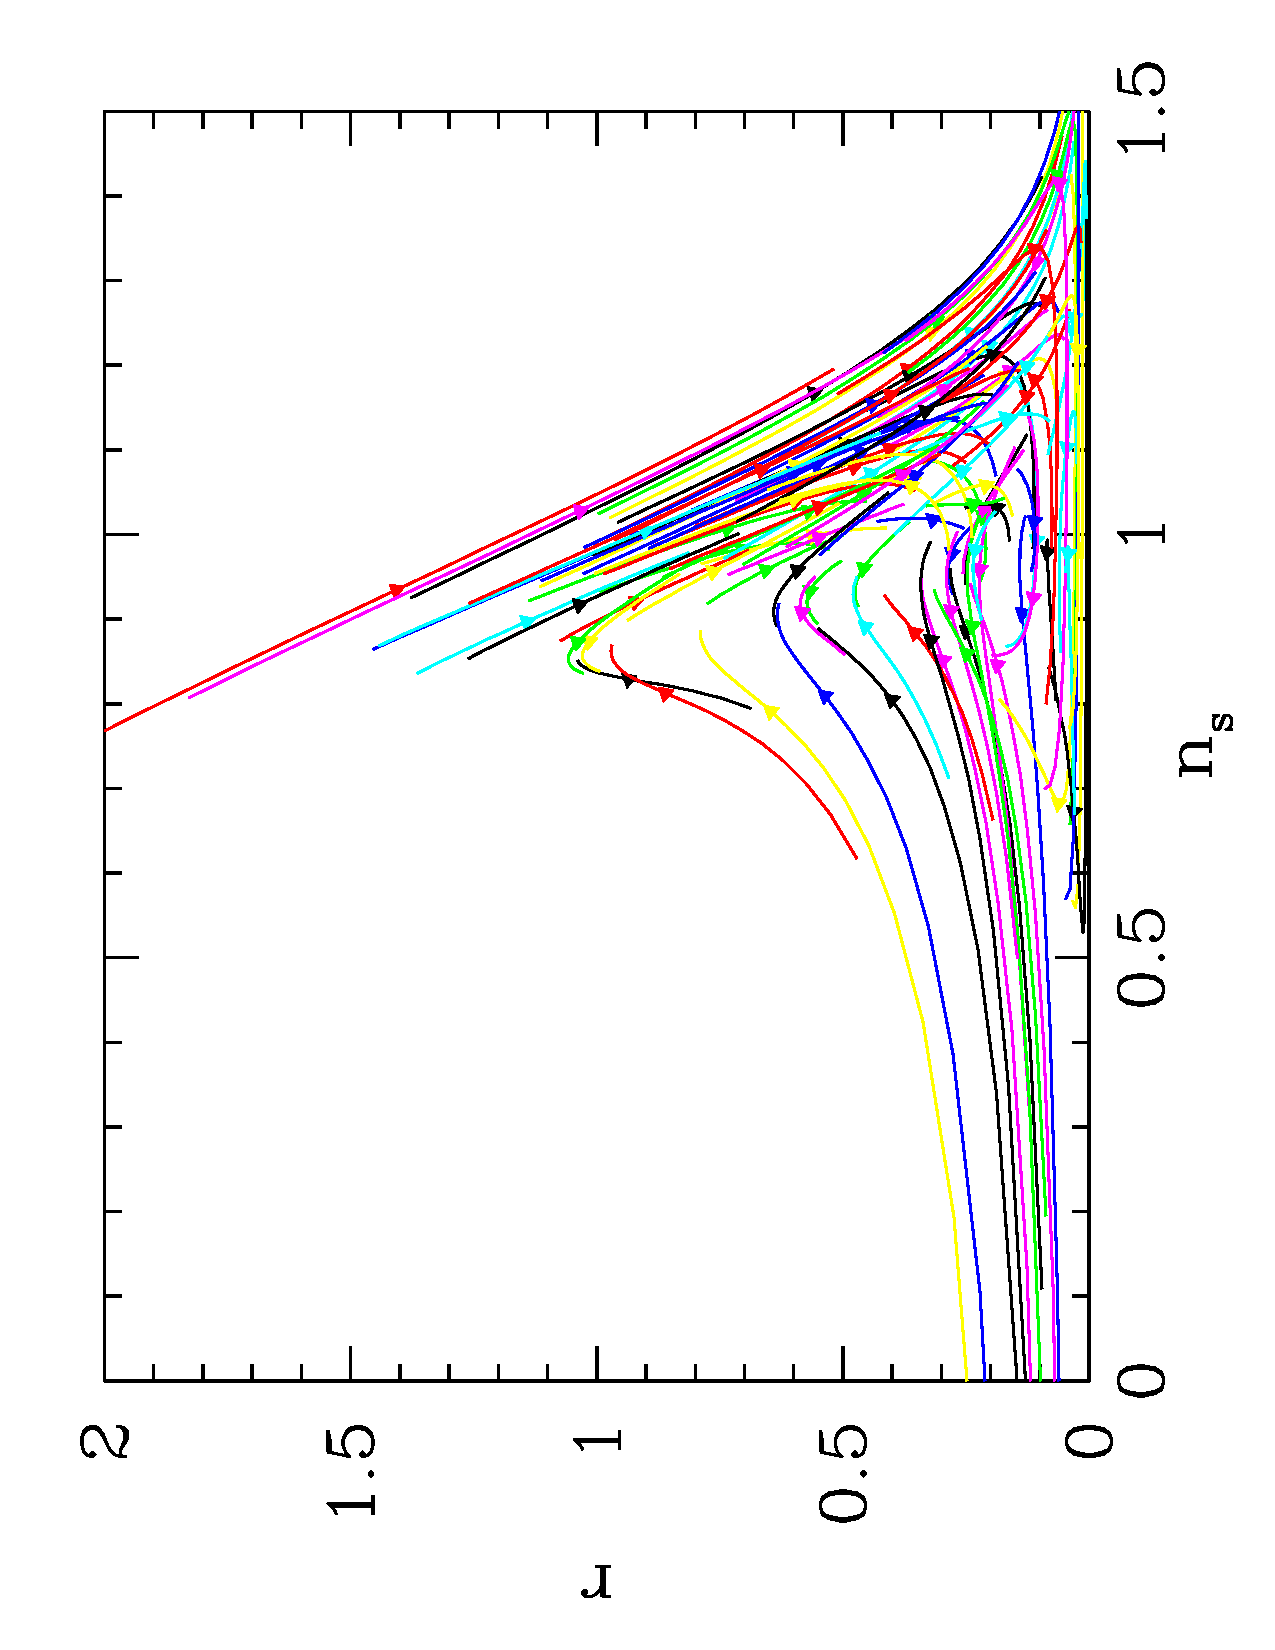
\includegraphics[angle=270, width=0.9\linewidth]{movingpoints_sm}
  \end{center}
  \caption[Flow of observables with varying $N$]{Flow along a random
  selection of the inflationary trajectories in the $n_s$ {\it vs.}
  $r$ plane during 10 $e$-folds. The trajectories were generated as
  seventh order Chebyshev expansions of $\epsilon(N)$. Different
  colors denote different trajectories.}
  \label{fig:movingpoints}
\end{figure}

\subsection{Trajectory functions}
In view of the above we examine in this work a bottom-up approach to
model building using the generalized trajectory picture. In our
approach, all fundamental quantities such as the tensor and scalar
power spectra or slow roll ``parameter'' $\epsilon$ are regarded as
trajectories, with a suitable choice of time variable such that there
are no ambiguities about the location of observable quantities while
at the same time capturing all essential dynamics. Instead of using
the traditional parameterization to characterize the primordial power
spectra, the trajectory functions are constrained directly using
standard parameter estimation packages employing Markov Chain Monte
Carlo (MCMC) methods. 

There are many possible choices for the trajectory function,
$\epsilon$, $\pscalar$, $\ptensor$, etc., with the only
criterion that one can map the trajectory function to the scalar and
tensor power spectra. For example, the trajectory function $\epsilon$
encodes all information about single field inflationary models as well
as (neglecting the influence of isocurvature perturbations) gentle
multiple field model in the sense that a sufficiently well-behaved
dynamics can be cast in terms of an effective single field
model. Mapping $\epsilon$ trajectories to observables requires an
integration step. Selecting the power spectra $\pscalar$ and
$\ptensor$ themselves as the trajectory functions offers more
flexibility, not only allowing for a non-monotonic tensor power
spectrum but also not relying on the single field approximation.  In
this paper we will focus on the choice of $\pscalar$ and
$\ptensor$ as trajectory functions and also explore the choice of
$\epsilon$ trajectories.

Different choices of trajectory functions come with different
priors. Indeed, as we point out in this work, a discussion of implied
priors is integral to this type of bottom-up approach and must be
discussed at length. The scalar (tensor) power $\pscalar$
($\ptensor$) are constrained to be strictly positive, while
$\epsilon$ is confined to lie in $\epsilon\in[0,1]$. Using $\epsilon$
trajectories implies single field inflation, a rather complex prior on
the allowed trajectories. Furthermore, there is the choice of measure
in sampling the chosen trajectories which can be linear or non-linear
in the chosen coefficients.

The different priors will sample the functional space of trajectories
with different measures. Depending on the quality of observational
data this will be reflected in the posterior space of traditional
observables. In particular the value of $r$ is strongly influenced by
the choice of trajectory function and the prior distribution of the
trajectory values. As we will show, although one can choose a uniform
prior in the original expansion coefficients, the mapping through to
final parameters is non-trivial and generally results in non-flat
priors which in some cases can be quite extreme \cite{Peiris:2006sj,
  Peiris:2006ug} with a resulting potential for misrepresentation of
observational constraints.

When working in this type of bottom-up approach, constraints are
imposed directly on the space of trajectories and the traditional
parameters become only ancillary products which should not be over
interpreted. The focus is shifted instead to the functional
reconstruction of the trajectories being considered, ${\cal P}_s$ and
${\cal P}_t$ in this case. Ultimately the approach can be extended to
reconstructing a fundamental trajectory such as $\epsilon(\ln k)$
which leads to direct constraints on the shape of the inflationary
potential.

The approach also requires a choice of parameterizing time along the
trajectory. A natural choice for this is the wave number
$k$ itself. As physical time evolves, modes of decreasing comoving
wavelength are stretched outside the horizon, crossing into the
super-horizon region when $k=aH$. This leads to the relation $d\ln k =
(1-\epsilon) H dt$, where $k$ is the comoving wave number of the mode
crossing the horizon, $t$ is the physical time, and
$\epsilon=-\frac{\dot{H}}{H^2}$ (where $\dot{H}=\frac{dH}{dt}$) which
makes $k$ a good time variable as long as the inflationary stage is
not interrupted by periods of non-exponential expansion with
$\epsilon\ge1$.

\section{Markov Chain Monte-Carlo}
Our Markov Chain Monte Carlo (MCMC) sampler is based on the publicly
available {\tt COSMOMC} \cite{Lewis:2002ah} and allows us to obtain
posterior distributions for the power spectra parameters as well as
the remaining background cosmological parameters. The first three are
related to abundances: $\omega_b\equiv\Omega_bh^2$, the physical
density of baryons, $\omega_c\equiv\Omega_ch^2$, the physical density
of cold dark matter, and $\theta\equiv100\ell_s^{-1}$, parameterizing
the angular scale $\ell_s^{-1}$ associated with sound crossing at
decoupling, which defines the overall position of the peak--dip
pattern and from which the cosmological constant $\Omega_\Lambda$ can
be derived. The remaining parameter, $\tau$, sets the amount of
reionization of the universe after recombination in the form of
Thomson scattering depth to decoupling. A flat universe theoretical
prior is reasonable to impose on inflation models, with the curvature
energy $\Omega_k = 1-\Omega_{\rm tot} \approx 0$.

There are data constraints beyond the CMB and LSS regions that are
only loosely determined, i.e. ``weak'' prior probabilities, informed
by broad brush stroke considerations, but still quite limiting. One is
that the Universe underwent significant inflation, translating at
lowest order to $0 < r < 16$ over the entire $k$ range within the
horizon. For the dynamical trajectories this corresponds to $0<
\epsilon < 1$, or equivalently an inflationary period that lasted for
a sufficient number of $e$-folds $N$.

Enough inflation implies that scales of topological structures cannot
be too small so that there is sufficient cosmic complexity to give
rise to life. Also, the amplitude of the power spectrum at high $k$
cannot be too large otherwise surviving primordial black holes (PBH)
formed in abundance. Another weak prior driven by the CMB data is that
the Compton ``optical'' depth cannot be too large or else there would
be no CMB fluctuations on small scales. This reflects in the formation
of the first ionizing stars and is more strongly restrictive than the
PBH constraint. The epoch of galaxy formation is also a constraint,
often used in a very broad way in anthropic arguments. The data on
high redshift galaxy abundances has improved enormously in recent
years and even with the uncertainties associated with gas and
radiation at early times can significantly constrain the power
spectrum. 

Improved observations narrow down the range of allowed variations. In
the eighties, upper limits on CMB fluctuations combined with a few LSS
constraints already restricted the allowed possibilities. The COBE
data further restricted what was allowed, and now in the era of WMAP
and higher resolution experiments, the possibilities for significant
variation from the standard model are much more limited.

Using the traditional parameterizations of the primordial power
spectra in terms of $A_s$ and $n_s$ and the most current data
including weak lensing, supernova and Lyman-$\alpha$ forest (see
Section~\ref{sec:data_sets}), current constraints on the
basic 6-parameter model are given in
Table~\ref{tab:marginalized_posteriors}, most notably
$n_s=0.962^{+0.011}_{-0.011}$. Including either $r$ or
$n_{\mathrm{run}}$, we find $r < 0.17 $ at the
95\% confidence limit with $n_{\mathrm{run}}=0$ and $r< 0.27$ with
$n_{\mathrm{run}} = -0.017^{+0.010}_{-0.010}$. Here we consider the
two parameter $r$ and $dn_s / d\ln k$ extension to the base model.
\begin{table}
  \begin{center} % or you can use \centering to remove the blank line between caption and table 
  \caption{The 68.3\% CL constraints on cosmological parameters (for
  $r$ the 68.3\%CL and 95.4\% CL upperbounds are shown). A
  $\Lambda$CDM model with $n_t=0$ has been assumed. For simplicity we
  have used the same pivot $k_{\rm pivot}=0.002\,{\rm Mpc}^{-1}$ for
  both scalar and tensor spectra. The data sets used here are
  described in Section~\ref{sec:spectral_trajectories}.}
   \label{tab:marginalized_posteriors}
   \begin{tabular}{ccc}
   \hline
    & with $n_{\rm run}$ & without $n_{\rm run}$ \\
    \hline
     $ \Omega_b h^2 $ & $0.02262^{+0.00043}_{-0.00044}$ & $0.02260^{+0.00044}_{-0.00044}$ \\
     $ \Omega_c h^2 $ & $0.1179^{+0.0020}_{-0.0020}$ & $0.1171^{+0.0019}_{-0.0019}$ \\
     $ \theta $ & $1.0425^{+0.0019}_{-0.0020}$ & $1.0420^{+0.0019}_{-0.0019}$ \\
     $ \tau $ & $0.094^{+0.015}_{-0.014}$ & $0.090^{+0.014}_{-0.014}$ \\
     $ n_s $ & $1.006^{+0.029}_{-0.029}$ & $0.962^{+0.011}_{-0.011}$ \\
     $ n_{\rm run} $ & $-0.017^{+0.010}_{-0.010}$ & \nodata \\
     $ \ln(10^{10}A_s) $ & $3.184^{+0.043}_{-0.047}$ & $3.226^{+0.033}_{-0.034}$ \\
     $ r $ & $0.0000^{+0.14+0.27}$ & $0.0000^{+0.08+0.17}$ \\
     $ \Omega_m $ & $0.293^{+0.012}_{-0.011}$ & $0.290^{+0.011}_{-0.010}$ \\
     $ \sigma_8 $ & $0.844^{+0.014}_{-0.014}$ & $0.843^{+0.014}_{-0.016}$ \\
     $ z_{\rm re} $ & $11.2^{+1.2}_{-1.2}$ & $10.8^{+1.2}_{-1.2}$ \\
     $ H_0 $ & $69.3^{+1.0}_{-1.0}$ & $69.4^{+1.0}_{-1.0}$ \\
   \hline
   \end{tabular}
   \end{center}  % if you use \centering, remove this line
\end{table}

\section{Data Sets}\label{sec:data_sets}
Before we proceed, we give a brief overview over the data sets that we
use in this paper. Besides current data sets, we also elaborate on
forecasts for future experiments.
\begin{itemize}
\item {\it Cosmic Microwave Background (CMB)} 

Our complete CMB data sets include WMAP-7yr
\cite{Komatsu2010,Jarosik2010}, ACT \cite{Fowler2010}, BICEP
\cite{Chiang2009}, QUaD \cite{Castro2009}, ACBAR
\cite{Reichardt2008,Kuo2006,Runyan2003, Goldstein2003}, CBI
\cite{Sievers2007,Readhead2004a,Readhead2004b,Pearson2003}, BOOMERANG
\cite{Jones2006,Piacentini2006,Montroy2006}, VSA \cite{Dickinson2004},
and MAXIMA \cite{Hanany2000}. For high-ell CMB experiments we have
used the Sunyaev-Zel'dovich (SZ) secondary anisotropy
\cite{Sunyaev1972,Sunyaev1980} template \cite{Bond2005}, but other
choices of SZ template are certainly possible \cite{Komatsu2002,
  Sehgal2009, Battaglia2010}. We treat the multiplier of the SZ
template as a free nuisance parameter $A_{\rm SZ}$ and marginalize
over it, making the cosmological parameters insensitive to the choice
of SZ template. The CMB lensing contribution is included when we
calculate CMB power spectra.

\item{\it Type Ia Supernova (SN)}

We use the \cite{Kessler2009} data set, which have combined the
SDSS-II SN samples with the data from the ESSENCE project
\cite{Miknaitis2007, Wood-Vasey2007}, the Supernova Legacy Survey
(SNLS) \cite{Astier2006}, the Hubble Space Telescope (HST)
\cite{Garnavich1998, Knop2003,Riess2004,Riess2007}, and a compilation
of nearby SN measurements. Two light curve fitting methods, MLCS2K2
and SALT-II, are employed in \cite{Kessler2009}. The different
assumptions about the nature of the SN color variation lead to a
significant discrepancy in dark energy parameters. Since we are only
interested in primordial power spectra and assuming a cosmological
constant, our choice of SALT-II filter throughoutt this paper does not
have significant impact on our results.

\item{\it Large Scale Structure (LSS)}

The LSS data used in this paper is the power spectrum of the Sloan
Digital Sky Survey Data Release 7 (SDSS-DR7) Luminous Red Galaxy (LRG)
samples \cite{Reid2009}. 

\item{\it Weak Lensing (WL)}

Five WL data sets are used in this paper. The effective survey area
$A_{\rm eff}$ and galaxy number density $n_{\rm eff}$ of
each survey are listed in Table~\ref{tab:wldata}.

\begin{table}
\begin{center}
  \caption{Weak Lensing Data Sets}
  \begin{tabular}{lll}
    \hline
    Data sets & $A_{\textrm{eff}}$ (deg$^2$)  &  $n_{\rm eff}$  (arcmin$^{-2}$) \\
    \hline
    COSMOS\cite{Massey2007,Lesgourgues2007}  & 1.6 & 40\\
    CFHTLS-wide\cite{Hoekstra2006,Schimd2007}& 22 & 12 \\
    GaBODS\cite{Hoekstra2002a,Hoekstra2002b} & 13 & 12.5 \\
    RCS\cite{Hoekstra2002a,Hoekstra2002b} & 53 & 8 \\
    VIRMOS-DESCART\cite{Van-Waerbeke2005,Schimd2007} & 8.5 &  15 \\
    \hline
  \end{tabular}
  \label{tab:wldata}
\end{center}
\end{table}

For the COSMOS data, we use the CosmoMC plug-in written by Julien
Lesgourgues \cite{Lesgourgues2007}. For the other four weak lensing
data sets we use the covariance matrices given
by Benjamin \etal \cite{Benjamin2007}. To calculate the likelihood we wrote a
CosmoMC plug-in code. We take the best fit parameters
$\alpha,\beta,z_0$ for $n(z)\propto
(z/z_0)^\alpha \exp{\left[-(z/z_0)^\beta\right]}$, and marginalize
over $z_0$, assuming a Gaussian prior with a width such that the mean
redshift $z_m$ has an uncertainty of $0.03(1+z_m)$. We have checked
that further marginalizing over the remaining $n(z)$ parameters
$\alpha$ and $\beta$ has no significant
impact \cite{Amigo2008,HBK2010}. We use the Halofit
formula \cite{Smith2003} to map the linear matter power spectrum to
nonlinear power spectrum. Because we are considering non-standard
forms of primordial spectra, the Halofit formula can be inaccurate ,
potentially washing out bump features by non-linear dynamics). To
model this additional uncertainty, we introduce two nuisance
parameters $\alpha_h$ and $\beta_h$
\begin{eqnarray}
\ln P_{\rm nl} &=& e^{-k^2r_{\rm nl}^2} \ln P_{\rm halofit} +  \left(1-e^{-k^2r_{\rm nl}^2}\right) \nonumber \\
       &&\, \times\left( \ln P_{\rm smooth} + \alpha_h + \beta_h k r_{\rm nl}\right) \ , \label{halofit_fix}
\end{eqnarray}
where $P_{\rm halofit}$ is calculated using the original halofit
formula code, with the nonlinear scale $r_{\rm nl}$ as a
byproduct. Here $\ln P_{\rm smooth}$ is obtained by fitting $\ln
P_{\rm halofit}$ as a quadratic function of $\ln k$ in the range where
$\ln (kr_{\rm nl})>-1$ and $k<{\rm Mpc}^{-1}$. We used priors
$-0.2<\alpha_h<0.2$ and $-0.2<\beta_h<0.2$, allowing about 20\%
uncertainty of $P_{\rm nl}$ on scales $\sim 1/r_{\rm nl}$, and even
larger uncertainties on smaller scales. By doing this we are
effectively discarding most of the information on non-linear scales,
with only a rough amplitude of the matter power spectrum being used.


\item{\it Lyman-$\alpha$ Forest (Ly$\alpha$)}

We use Ly$\alpha$ data sets given in McDonald \etal \cite{McDonald2005,McDonald2006}. To calculate the likelihood, we interpolate
the $\chi^2$ table in a three dimensional parameter space, where the
three parameters are amplitude, index, and the running of linear
matter power spectrum at pivot point $k_{\rm lya}=0.9 h$
Mpc$^{-1}$. To extract these parameters from more general power
spectra that are allowed in our parametrization, we perform a
quadratic fitting of $\ln P_{\rm matter}$ for $\ln k_{\rm lya}-1/2
< \ln k < \ln k_{\rm lya} + 1/2$, and marginalize over 2\% uncertainty
of the amplitude and 5\% uncertainty of the spectral index.

\end{itemize}

In addition to the most current catalog of cosmological data sets, we
consider in alternatively forcast data from forthcoming cosmic
surveys. The Planck satellite is expected to measure the CMB
temperature fluctuations to ultimate
accuracy \cite{book_PlanckBlue}. The EUCLID weak lensing survey will
probe large scale structure deep into redshift
$1.1$ \cite{book_EUCLIDYellow}, with possible extensiosn to much
higher redshift by 21-cm surveys such as the Canadian Hydrogen
Intensity Mapping Experiment (CHIME) \cite{book_CHIMEWhite}. The Joint
Dark Energy Mission (JDEM) will expand the current supernova catalog
by an order of magnitude \cite{DETF}. To model these forthcoming data
sets, we assume that the mapping between linear and nonlinear matter
power spectra is well understood (especially for the more general
power spectra we consider here). We hence directly apply the
likelihood codes and mock data simulation techniques that we used in
Ref.~\cite{HBK2010}, with no further modifications for more general
primordial spectra.

\section{Spectral Trajectories}\label{sec:spectral_trajectories}
As indicated in the introduction, we will first focus on the
reconstruction of the primordial power spectra while ignoring any
priors from mechanisms that would produce them. Specifically in this
section, we shall not assume a scalar field driving inflation,
i.e. the consistency condition between the scalar and tensor
perturbation spectra. Instead we vary the $\ptensor,
\pscalar$ (or some quantities related to them) as independent
spectral trajectory functions. Only observational data can and shall
decide whether a trajectory is permissible or not.

The power spectra are traditionally parameterized as
\begin{eqnarray}
  \ptensor=A_t \left(\frac{k}{k_p}\right)^{n_t}\, ,&& \pscalar=A_s\left(\frac{k}{k_p}\right)^{n_s-1}\, ,
\end{eqnarray}
where $A_{t, s}$ are the tensor and scalar amplitudes, and $n_{t, s}$
are the corresponding spectral indices which are generally assumed to
be constant. Common values for the position of the pivot point $k_{p}$
are $0.05\mpc^{-1}$ and $0.002\mpc^{-1}$. In this language, the
consistency relation is
$n_t=-\frac{\ptensor}{8\pscalar}$. Figure \ref{fig:r-ns}
shows the limits on the values of the tensor scalar ratio
$r\equiv\frac{\mathcal{P}_T}{\mathcal{P}_S}$ and the scalar spectral
index $n_s$. 

\begin{figure}
\centering
  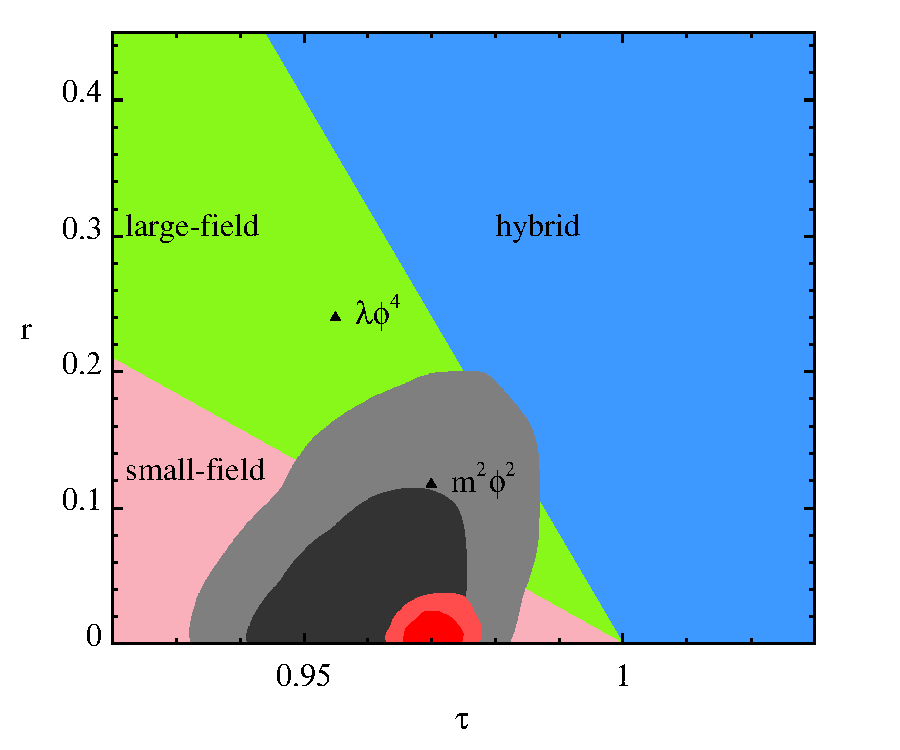
\includegraphics[width=0.9\linewidth]{ns_r_inf_models}
  \caption{Limits on the values of the tensor scalar ratio $r$ and
    scalar spectral index $n_s$ for current data (grey contours) as
    well as a forecast for Planck (red contours). Also displayed are
    the different classes of single scalar field theories covering
    this space of observables. Here $n_{\rm run}=0$ and $n_t=0$ are assumed.}
  \label{fig:r-ns}
\end{figure}

From a theoretical point of view, the running of the spectral index
can generally be non-zero, $n_{\mathrm{run}}=\frac{d n_s}{d\ln k}\neq
0$. Although recent observations do not see a significant probability
for non-zero running, one has to keep in mind that this result could
possibly be driven by an implicit prior in the choice of
parameterization. Different parameterizations might not conclusively
detect non-zero running, but they can show that the bounds on
$\left|n_{\mathrm{run}}\right|$ are larger than the standard
parameterization suggests.

The traditional parameterization of the power spectra with a constant
$n_s$ is motivated by the fact that a pure deSitter stage of inflation
has perfectly flat power spectra and that in many models of inflation
driven by a scalar field, the field is almost constant during
inflation, producing fluctuations with $n_s$ only slightly different
from unity. But these considerations are just a theoretical
bias. Observational data should be determining the parameters of the
primordial power spectra as unbiased as possible.

We will expand the trajectory function $f(x)=\mathcal{P}_{S,T}$ in
terms of basis functions $w_i$
\begin{eqnarray}
  f(x)&=&\sum_{i} f_i w_i(x)\, ,
\end{eqnarray}
where the functions $w_i(x)$ are either Chebyshev polynomials, a
suitable representation of B-splines or Hermite polynomials (see
Appendix~\ref{app:polynomials} for more details and a brief
introduction to both). By using high order expansions, we explore the
freedom that is in the data, while at the same time we shall keep an
eye on the effect of priors. 


The trajectory functions are subject to certain constraints, such as
positivity for the power spectra, or being confined in the interval
$[0,1]$ for the slow roll parameter $\epsilon$. Sampling the
coefficients and then rejecting the trajectories that do not fulfill
the constraints is both inefficient and -- more severely -- implies a
prior on the coefficients that is hard to overcome. Thus, the values
of the trajectories at the knots of the expansion should be sampled.

As we will see below, even this approach has some disadvantages. If
the data is not strong enough, the reconstructed trajectories might
show oscillatory features, or some residual implicit prior ,
e.g. positivity, might induce spurious detection of the tensor power
spectrum. As it is known beforehand that the currently available
observations do not possess enough power to constrain the tensors, we
shall parameterize $\ptensor$ at most by the tensor scalar ration $r$ and a
tensor index $n_t$.

As observational data is only available from the horizon size up to
the scale of Lyman-$\alpha$ clouds, we restrict the range in k-space over
which to expand the trajectories to $-9<\ln \left(k/{\rm Mpc}^{-1}\right)<1$. 

\subsection{Interpolation between seven knots} \label{sec:7knots}
First, we will discuss our results for a semi-blind expansion of
$\ln \pscalar$ using natural cubic spline interpolation between $7$
knots while parameterizing the tensor spectrum using $A_t$ and $n_t$
(with priors $A_t>0$ and $-0.1<n_t<0$). 

\subsubsection{Results for current data}
Figure~\ref{fig:7knot_Ps_Pt} shows the best-fit scalar (solid blue)
and tensor (solid red) power spectra together with trajectories from
within a $1$-$\sigma$ interval around the best-fit points (shown in
dashed blue/orange). While the tensor power spectrum is largely
unconstrained with $r(0.002\mpc^{-1})<0.89$ at $95.4\%$ CL, the scalar
power spectrum is somewhat better constrained -- which will have
profound implications for the spurious detection gravitational waves
when taking into account the consistency condition for single field
inflation below. However, the scalar spectrum is only well constrained
within the range $\goodkrange$, due to the presence of cosmic variance
on large scales and nonlinear structures on small scales. 

\begin{figure}
  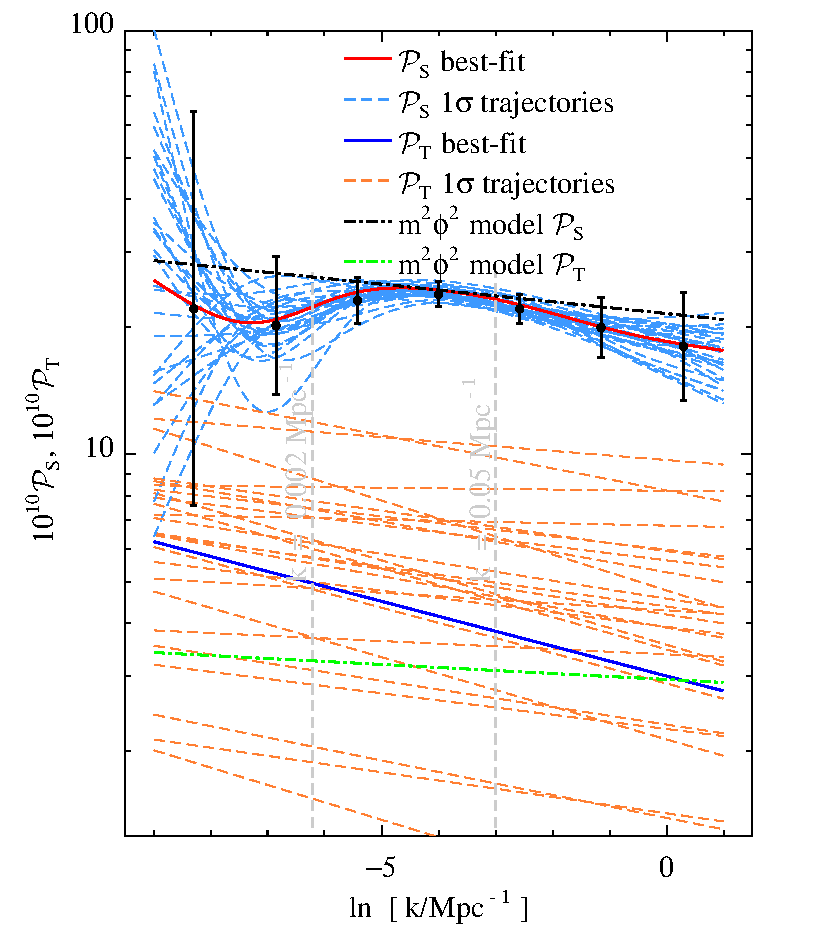
\includegraphics[width=0.9\linewidth]{p7cubicspline_traj11} 
  \caption{Reconstructed best fit scalar (solid red) and tensor (solid
  blue) power spectra using the current data. Also shown are the band
  powers obtained by convolving the power spectra with top-hat window
  functions in uniform $\ln k$ bins, with black error bars
  representing the $1\sigma$ uncertainties and correlation matrix
  shown in Figure~\ref{fig:band_band_correlations}. Trajectories from
  the $1\sigma$ interval around the best-fit points are shown as
  dashed blue and dashed orange lines for the scalars and tensors,
  respectively. The power spectra for $m^2\phi^2$ (dot-dashed black
  line for scalar and dot-dashed green line for tensor) agree pretty
  well with the reconstructed scalar spectra. The logarithm of the
  scalar spectrum was interpolated in cubic splines between $7$
  uniformly distributed $\ln k$ knots whereas the tensor spectrum was
  parameterized as $A_t \left(k/k_{\rm pivot}\right)^{n_t}$ with prior
  $-0.1<n_t<0$. At $95.4\%$CL, $r(0.002\mpc^{-1})
  <0.89$.}
  \label{fig:7knot_Ps_Pt}
\end{figure}

\begin{figure}
  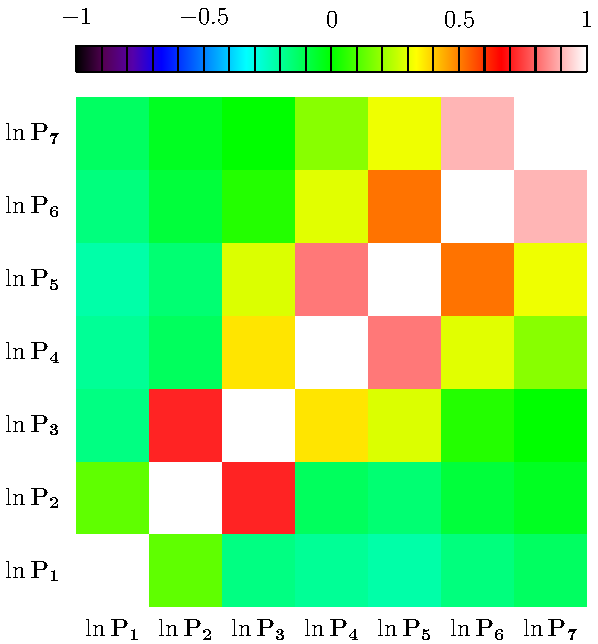
\includegraphics[width=0.9\linewidth]{p7cubicspline_correlation} 
  \caption{Correlation matrix of the reconstructed scalar power
  spectrum (see Figure~\ref{fig:7knot_Ps_Pt}).  The neighboring band
  powers are strongly correlated whereas those far away have almost no
  correlation.}  
  \label{fig:band_band_correlations}
\end{figure}

As can be seen in Figure~\ref{fig:7knot_Cl_TT_BB}, the response of the
$C_\ell$'s to the reconstructed primordial power spectra is consistent
with the uncertainties of the measured CMB angular power spectra
(including cosmic variance). Panel Figure~\ref{fig:7knot_Cl_TT_BB}(a)
shows the best-fit angular temperature autocorrelation function in
solid red, and trajectories from within a $1\sigma$ interval around
the best fit points in dashed blue. While on scales $\ell>20$, there
is only a small uncertainty in the scalar power spectrum, cosmic
variance leaves the angular scales $\ell<20$ rather unconstrained,
with strong deviations from the best fit trajectory possible. Note
that these wild excursions of the scalar power cannot be seen when
parameterizing $\pscalar$ with only an amplitude and a spectral index:
In this case, the constraints from scales $\goodkrange$ fix the local
slope of the spectrum quite tightly. On the other hand, the increased
freedom of the trajectories -- especially with larger number of nodal
points -- enables much stronger features in $\pscalar$.

\begin{figure*}
  (a)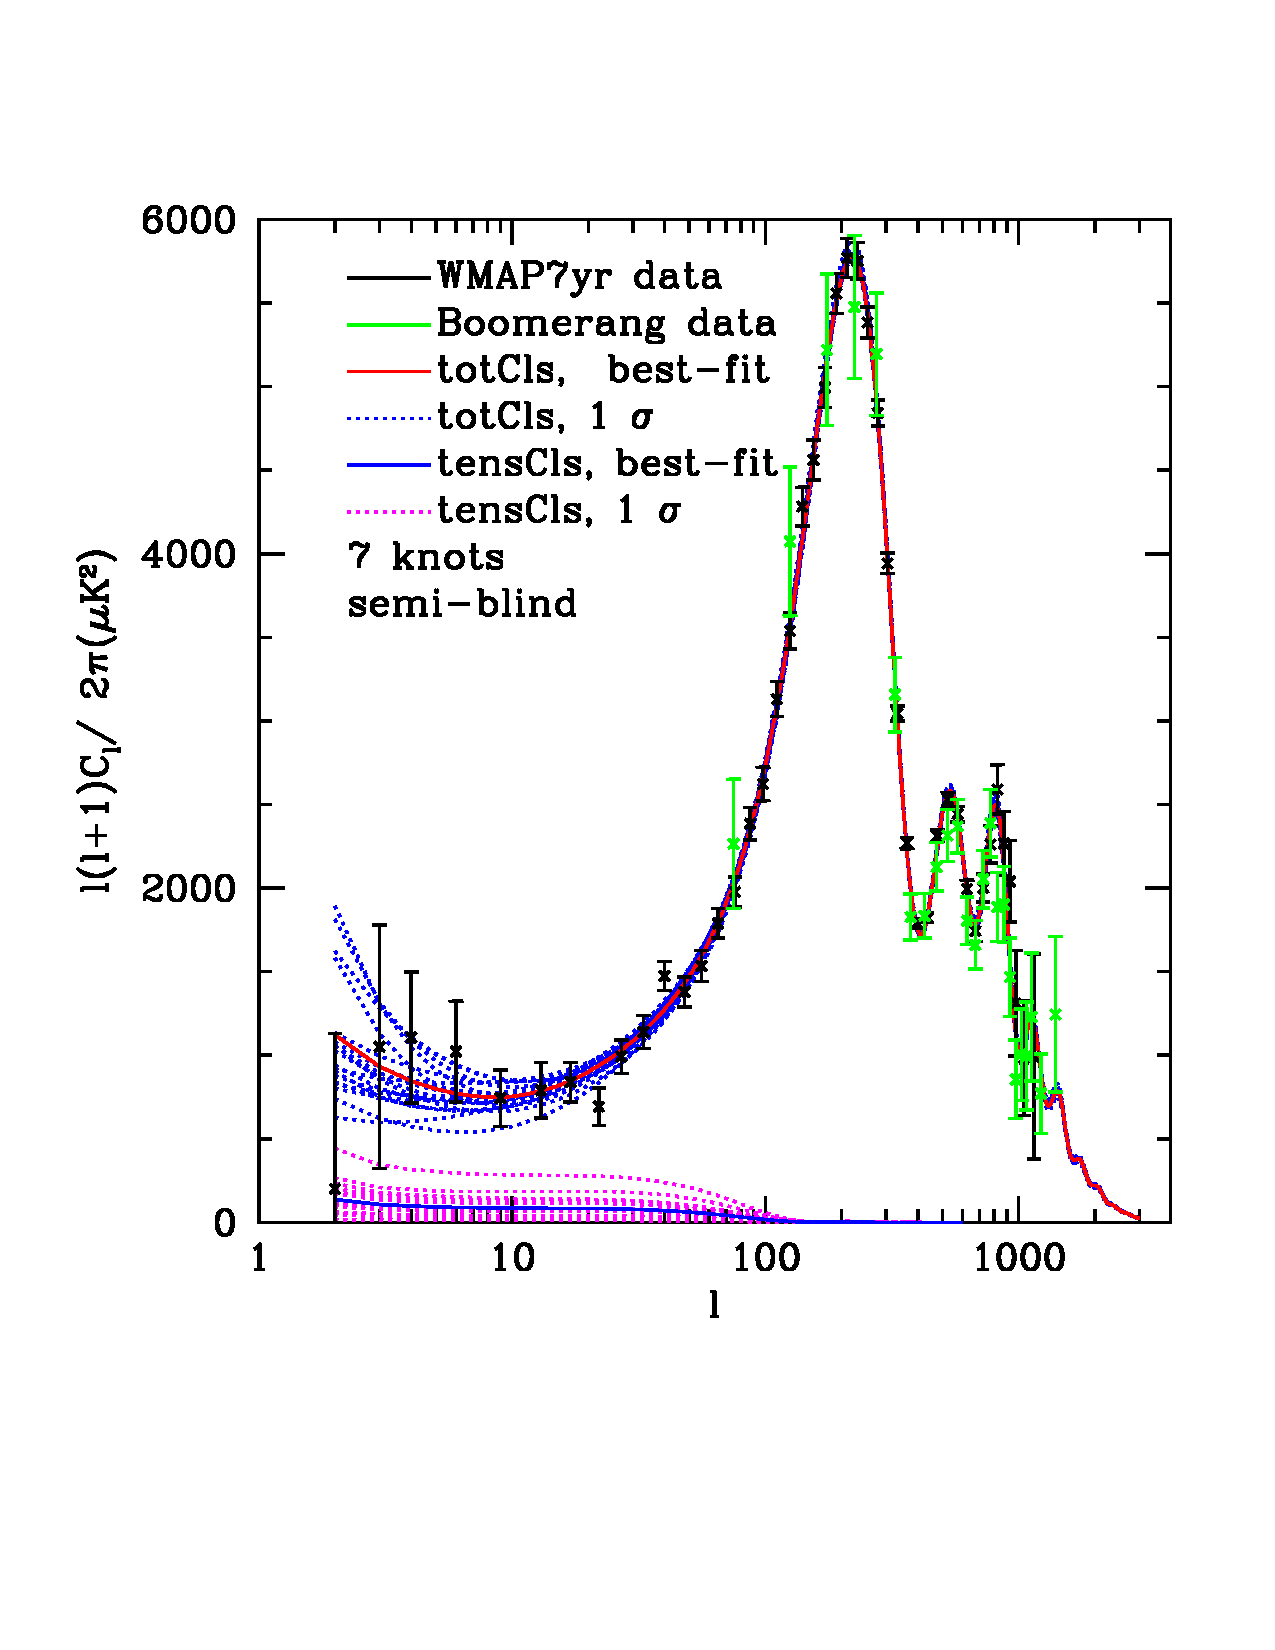
\includegraphics[width=0.45\linewidth]{p7cubicspline_TT}
  (b)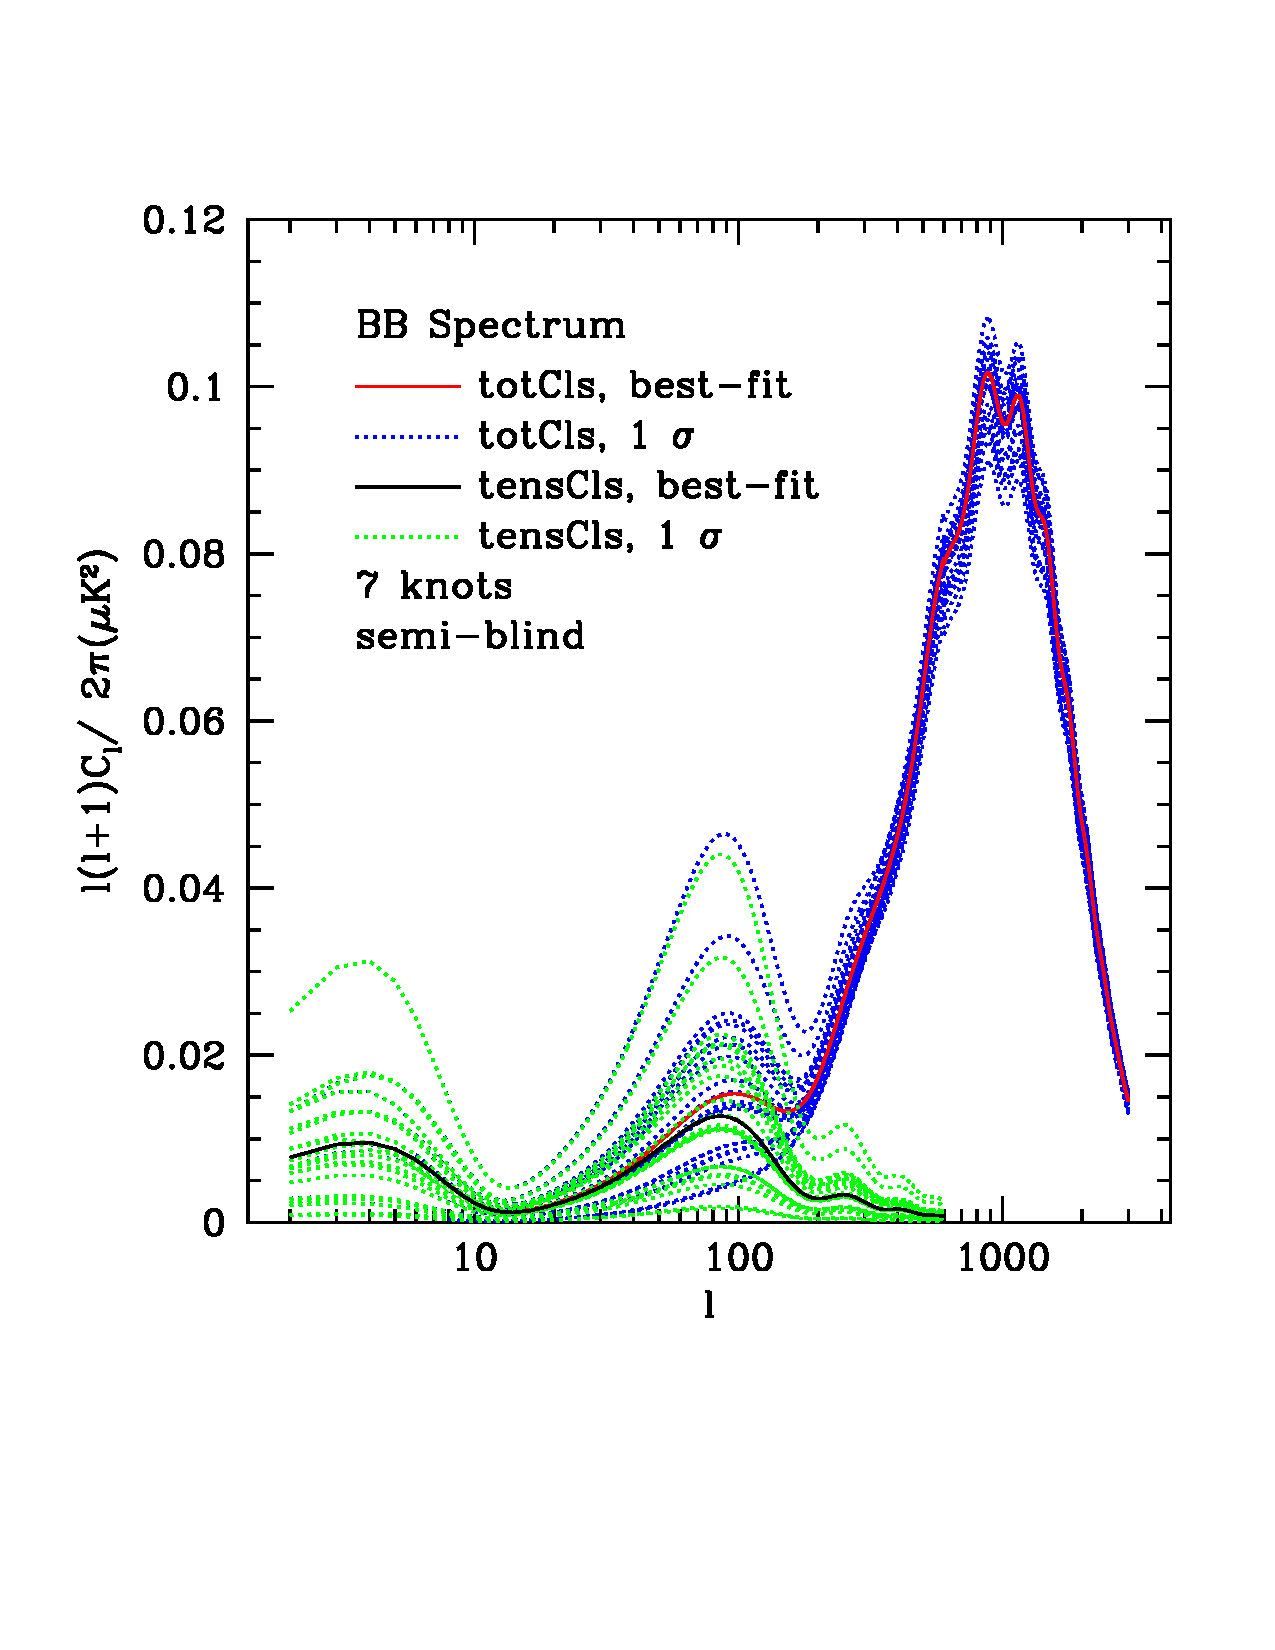
\includegraphics[width=0.45\linewidth]{p7cubicspline_BB}
  \caption{Response of the angular power spectrum $C_\ell$ for (a)
    temperature (TT) anisotropies and (b) B-mode polarization. The
    best fit trajectories are shown in solid red, while sample
    trajectories from within a $1\sigma$ interval around the best fit
    point are shown in dashed blue. Panel (a) shows the best fit
    contribution of the tensors to the TT spectrum in solid black as
    well as its $1\sigma$ variation (in dashed purple).}
  \label{fig:7knot_Cl_TT_BB}
\end{figure*}
Panel \ref{fig:7knot_Cl_TT_BB}(b) shows the B-mode polarization.  As
expected, the contribution to the $C_\ell^{BB}$ spectrum coming from
the primordial tensors (shown in solid black and dashed green) is
completely unconstrained from below and shows no signs of an
unambiguous detection.

\subsubsection{Principal Component Analysis}
Recently, principal component analysis (PCA, \cite{Huterer:2002hy})
has gained some attention \cite{Dvorkin:2010dn}. This is another way
of representing trajectories, however not as an expansion in a fixed
set of basis functions. Instead, the basis functions vary depending on
the error bars of the data. They are determined as the eigenfunctions
of the covariance matrix of either the observable data points
themselves or some derived quantities. So while in intermediate steps,
the trajectories under consideration are still expanded in basis
functions, the final results are represented as the eigenmodes of
their coefficients' covariance matrix, with only the best-constrained
eigenmodes kept for analysis. In Figure~\ref{fig:eigenmodes} we show
the eigenmodes of a $10$ knot cubic spline interpolation of
$1-n_s$. After constraining the values of the trajectories at the
knots and obtaining their covariance matrix, we diagonalize this
matrix and only display the first three eigenmodes which have
eigenvalues $0.015^2, 0.017^2, 0.032^2$. They are peaked
around $\ln \frac{k}{\mpc^{-1}}=-3.8, -4.5$, and $-2.5\mpc^{-1}$,
corresponding to $\ell=160,80, 580$. 
\zq{The first eigen mode is close to a single peak, $\ell = 160$ (close to the first CMB peak) makes sense. The second and third eigen modes have multiple peaks. We should probably not say they are peaked around some $\ell$.}
%\pmv{These $\ell$ values don't make much sense. I would have expected the location of the first and second peak in the $C_{\ell}$'s. Or should I not use the peaks of the eigenmodes but some sort of central value?}

\begin{figure}
  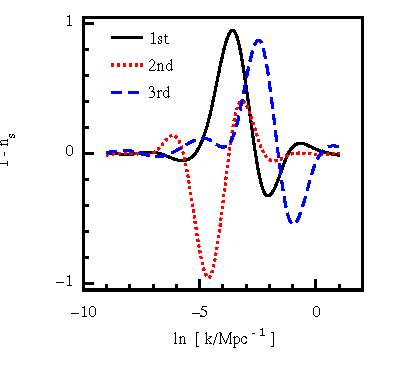
\includegraphics[width=0.9\linewidth]{p10nscubicspline_PCA} 
  \caption{The first (solid black), second (dot red) and third (dashed
  blue) eigen modes of $1-n_s$. Here we have done natural cubic spline
  interpolations of $2\epsilon + d\ln\epsilon/d\ln k\approx 1-n_s$
  between 10 knots, assuming single-field inflation.}
  \label{fig:eigenmodes}
\end{figure}
Alternatively, one might perform this eigenmode analysis for all other
trajectory expansions. However, the bottom line is that the PCA --
while providing a useful measure of the amount of information in the
data -- does obscure the influence of priors, something that is much
more readily visible in the trajectory approach.

\subsubsection{Results for forecasts}
In parallel we discuss forecasting future experiments using the freely
varying $\pscalar,\ptensor$ trajectories. Besides the interest in
forecasts in their own right, this also serves as a further exercise
that shall convince us that we did not introduce any serious bugs into
CosmoMC. We will examine two different fiducial models, both with the
same fiducial amplitude and scalar spectral index $n_s=0.97$, but
different in tensor scalar ratio $r$.

First, we reconstruct the inflationary trajectories $\pscalar,
\ptensor$ for a fiducial $V(\phi)=m^2\phi^2$ model of inflation, with
a tensor scalar ratio $r(0.002\mpc^{-1})=0.13$, see
Figure~\ref{fig:fc_p7m2phi2}(a). The scalar perturbations are well
recovered: the solid red best fit trajectory and the dashed blue
$1\sigma$ trajectories fit nicely to the dashed dotted black fiducial
$\pscalar$. The fiducial amplitude of the tensors (shown in dashed
dotted green) is found with about $1\sigma$ precision. However the
slope of the tensors $n_t$ seems quite off, and essentially is driven
by the chosen prior $-0.1<n_t<0$.  Even with data sets that will be
available in the near future, the tensor spectral index will not be
constrained. Only experiments like the big bang observer (BBO) will be
able to shed more light on the shape of the tensor power spectrum.

\begin{figure*}
  (a)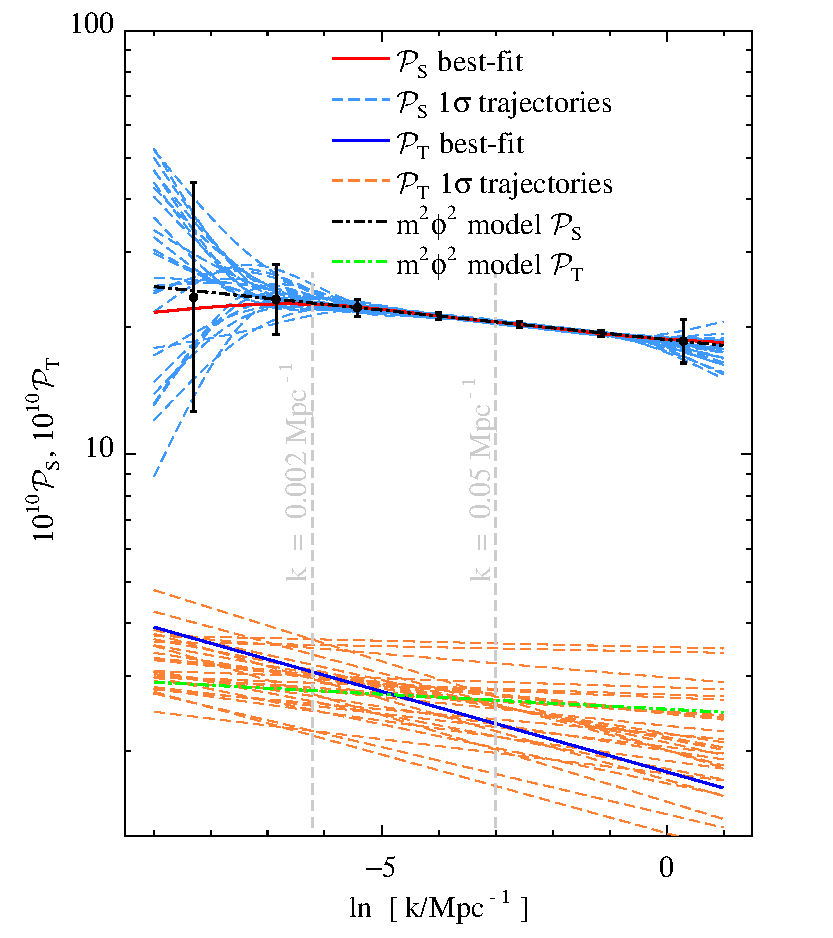
\includegraphics[width=0.45\linewidth]{fc_p7m2phi2_traj11}
  (b)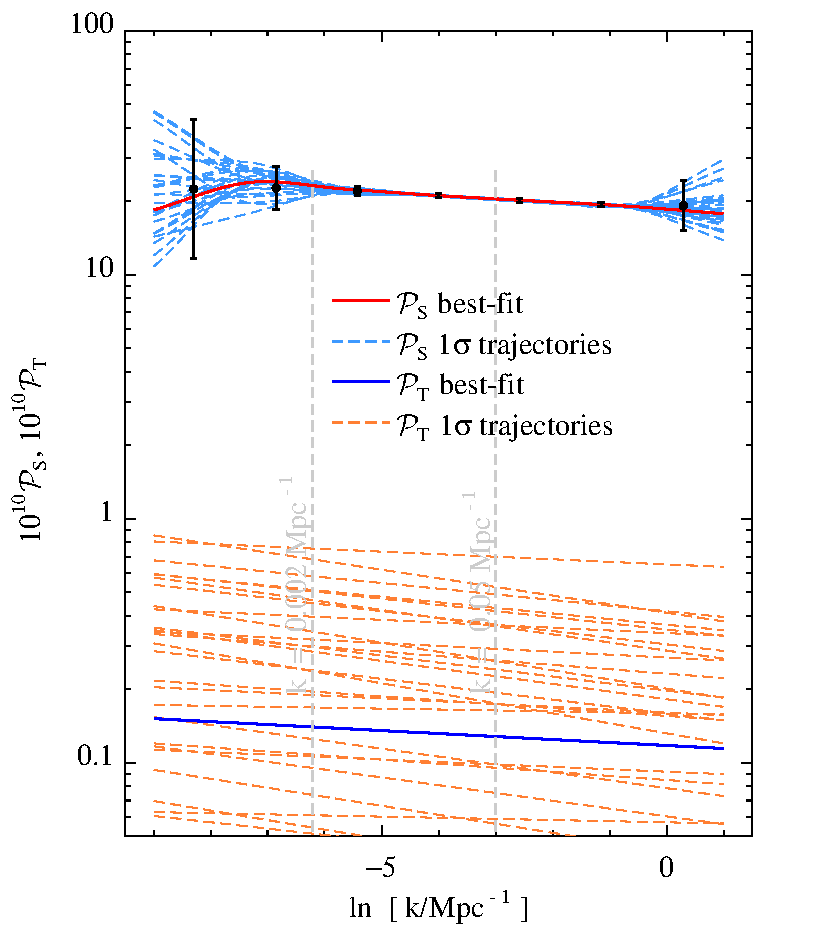
\includegraphics[width=0.45\linewidth]{fc_p7hermite_traj11}
  \caption{Reconstruction of (a) the fiducial $m^2\phi^2$ inflationary
    model with $r=0.13$ and (b) a fiducial model with $r=0$, assuming
    $2.5$ years of Planck data. The solid red/ dashed blue line shows
    the best fit/ $1\sigma$ $\pscalar$ trajectories. The solid blue/
    dashed red line shows the best fit/ $1\sigma$ $\ptensor$
    trajectory. The scalars/ tensors of the fiducial model in (a) are
    shown as dashed dotted black/ green line. For both models, the
    $\pscalar$ reconstruction works spectacularly well. In (a), the
    reconstructed amplitude of $\ptensor$ agrees within errors bars,
    however the slope seems quite off. The logarithm of scalar
    spectrum was interpolated in cubic splines (panel (a)) or cubic
    hermite (panel (b)) between $7$ uniformly distributed $\ln k$
    knots. The tensor spectrum was parameterized as
    $A_t \left(k/k_{\rm pivot}\right)^{n_t}$ with prior
    $-0.1<n_t<0$. } 
  \label{fig:fc_p7m2phi2}
\end{figure*}
Secondly, we reconstruct a fiducial model with $r=0$ in
Figure~\ref{fig:fc_p7m2phi2}(b). Again, the scalar spectrum is
beautifully recovered. Only an upper limit on the tensors is found,
consistent with $r=0$. To test the dependence of our results of the
choice of interpolation method, in Figure~\ref{fig:fc_p7m2phi2}(b) we
have used a different interpolation method -- the monotonic cubic
Hermite interpolation.  The technical details of various interpolation
methods we employed are given in the Appendix.

\subsection{Effects of changing the details of the trajectory expansion}

While the reconstructed power spectra do not differ much when using
monotonic cubic Hermite interpolation (or an expansion Chebyshev
polynomials) instead of cubic splines, varying the priors results in
dramatic changes in the power spectra. Priors can be changed either
explicitly (e.g. assuming a uniform prior in $\ln A_t$ instead of
$A_t$) or implicitly (by sampling the coefficients of the spline/
Chebyshev expansion instead of the trajectory values at the
knots). The effects of changing the priors explicitly are rather
trivial. For example, a uniform prior in $\ln A_t$ leads to much
tighter upper limit on the tensor spectrum.  Other changes to the
details of the trajectory expansions are more subtle. We will discuss
some notable examples in the following.

\subsubsection{Connection to the standard parameterization}

In order to connect our work to the standard parameterization, we
performed an order $2$ natural cubic spline expansion (i.e. linear
interpolation) for $\ln \pscalar$ which has the same number of degrees
of freedom as the standard parameterization using $\ln A_s, n_s$. It
is trivial to convert the values of $\ln \pscalar$ at the $2$ knots to
$\ln A_s, n_s$. Figure~\ref{fig:2knot_Ps_Pt} shows the reconstructed
primordial trajectories for $\pscalar$ trajectory with 2 knots,
employing the same color code as Figure~\ref{fig:7knot_Ps_Pt}.
\begin{figure}
  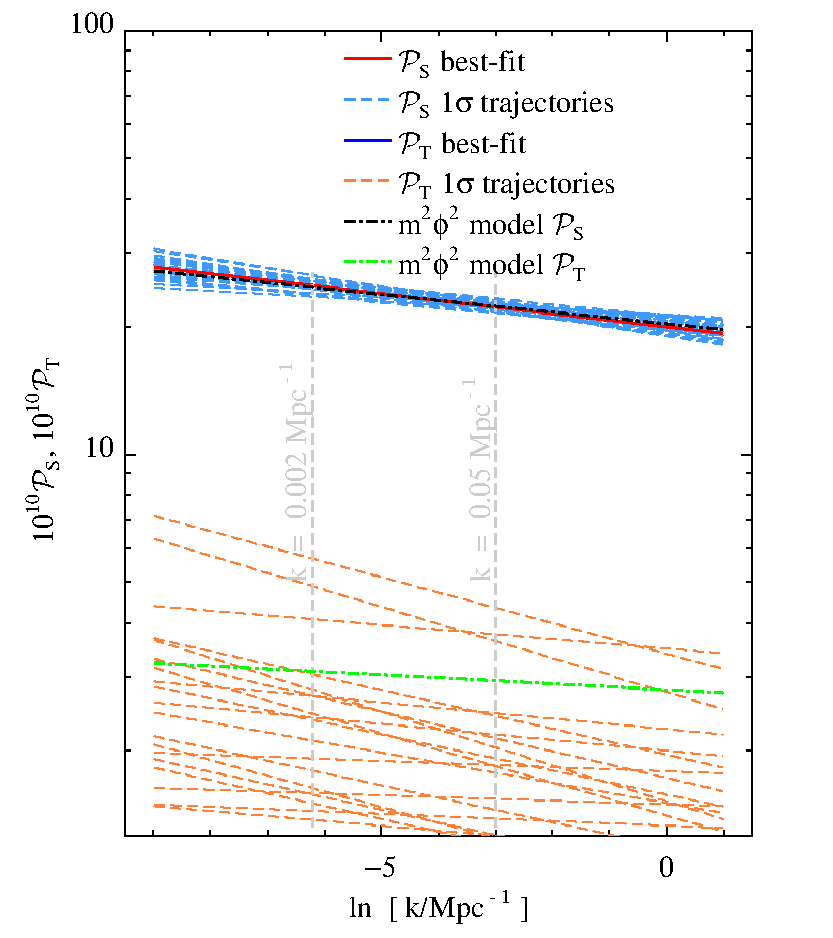
\includegraphics[width=0.9\linewidth]{p2cubicspline_traj11}
  \caption{The reconstructed scalar and tensor power spectrum, using
    natural cubic splines with $2$ nodal points for $\pscalar$ and $r,
    n_t$ (with priors $r>0$ and $-0.1<n_t<0$) for
    $\ptensor$.}
  \label{fig:2knot_Ps_Pt}
\end{figure}
Not surprisingly, the resulting values for
$\ln\left(10^{10}A_s\right)=3.220^{+0.037}_{-0.036}$,
$n_s=0.966^{+0.011}_{-0.012}$ are in excellent agreement with the
values obtained by the standard parameterization (with $r>0$ and
$-0.1<n_t<0$)
$\ln\left(10^{10}A_s^{\mathrm{std}}\right)=3.226^{+0.033}_{-0.034},
n_s^{\mathrm{std}}=0.962^{+0.011}_{-0.011}$. The small differences
come from a slight change in priors due to the different
parameterizations.


\subsubsection{Oscillations from too much freedom}

Having made the connection with the standard parameterization by
employing a 2-knot natural cubic spline, we now examine the effects of
allowing more freedom for the scalar spectrum. As example we will use
a 11-knot cubic spline expansion for $\ln \pscalar$.
\begin{figure}
  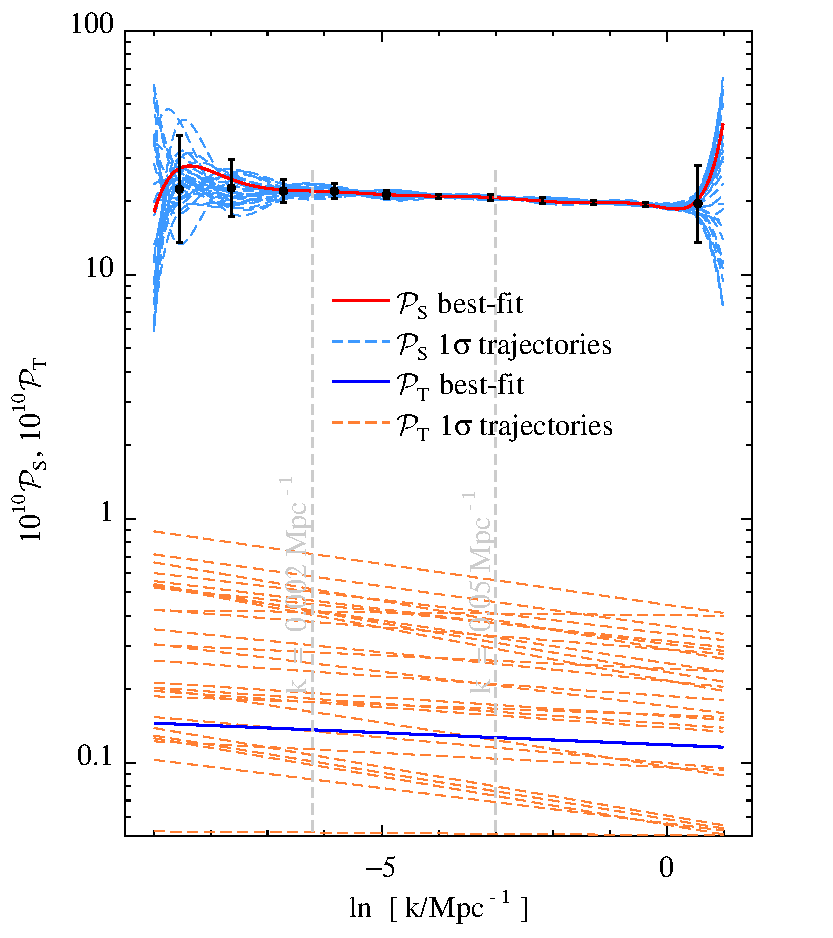
\includegraphics[width=0.9\linewidth]{fc_p11cubicspline_traj11} 
  \caption{Increasing the number of knots for $\pscalar$ leads to
  oscillations. Mock data with fiducial $r=0$ has been used.}
 \label{fig:11knot_Ps_Pt}
\end{figure}
In Figure~\ref{fig:11knot_Ps_Pt}, we see the presence of oscillatory
features, particularly on scales where $\pscalar$ is not well
determined.  They are due to an excessive number of degrees of freedom
in the parametrization.  However, when mapped into $C_\ell$ space, the
resulting angular power spectra agree with observations within (cosmic
variance-dominated) error bars.

\subsubsection{Tensor power spectrum driven by prior}

As a final example of the effects of different priors, we take a look
at the impact of increasing the number of knots for the tensor power
spectrum interpolation. The monotocity condition $d\ln \ptensor/d\ln
k<0$ required by inflation is applied to the $\ptensor$ trajectories.
Figure~\ref{fig:7knot_Ps_5knot_Pt} shows that an increase in the
allowed complexity for the tensor (from 2 degrees of freedom to 5)
leads to detection of $\ptensor$ on large scales.  This detection is
known to be false, because the fiducial model has $r=0$.  The favored
larger amplitude of $\ptensor$ on large scales is driven by the
monotonicity prior, as clearly visualized in the figure.

\begin{figure}
  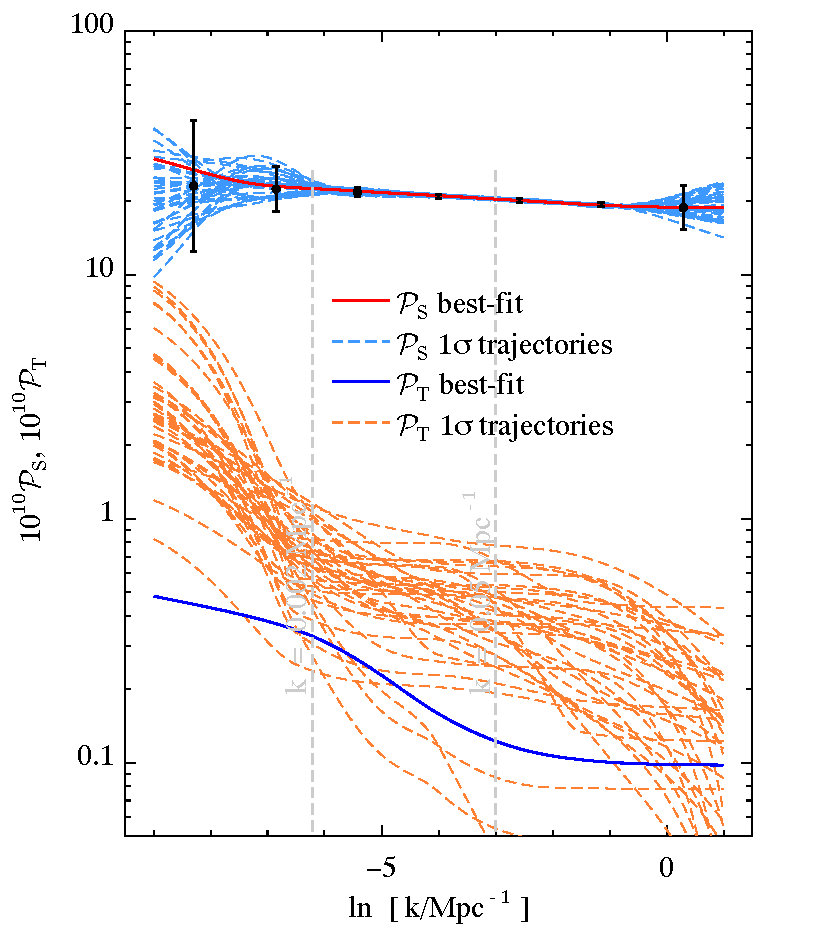
\includegraphics[width=0.9\linewidth]{fc_p7p5hermite_traj11}
  \caption{Increasing the number of knots for the tensor power
  spectrum from 2 degrees of freedom to 5 degrees of freedom, with the
  monotocity condition $d\ln \ptensor/d\ln k<0$ applied. Mock data
  with fiducial $r=0$ have been used here. The uncertainty in the
  tensor spectrum is driven by the priors.}
  \label{fig:7knot_Ps_5knot_Pt}
\end{figure}

Alternatively, one can easily see the influence of the prior on the
reconstructed parameters when simulating data for a Planck or CMBPol
type experiment, see Figure~\ref{fig:rin_rout}. Reconstructing the
input values $r_{\mathrm{reconstructed}}$ of the input tensor scalar
ration $r_{\mathrm{in}}$ shows that for at the limits of the
experiment -- for small enough values of $r_{\mathrm{in}}$,
e.g. $r_{\mathrm{in}}=0.0001$ for CMBPol -- the priors drive the
reconstructed value.  While for the $\pscalar, \ptensor$ trajectory
(black) the reconstructed value $r_{\mathrm{reconstructed}}$ is too
large, in the case of an $\epsilon$ (red) or $\ln\epsilon$ (blue)
trajectory, the error bars grow tremendously and the central value
shifts considerably.
\begin{figure*}
  (a)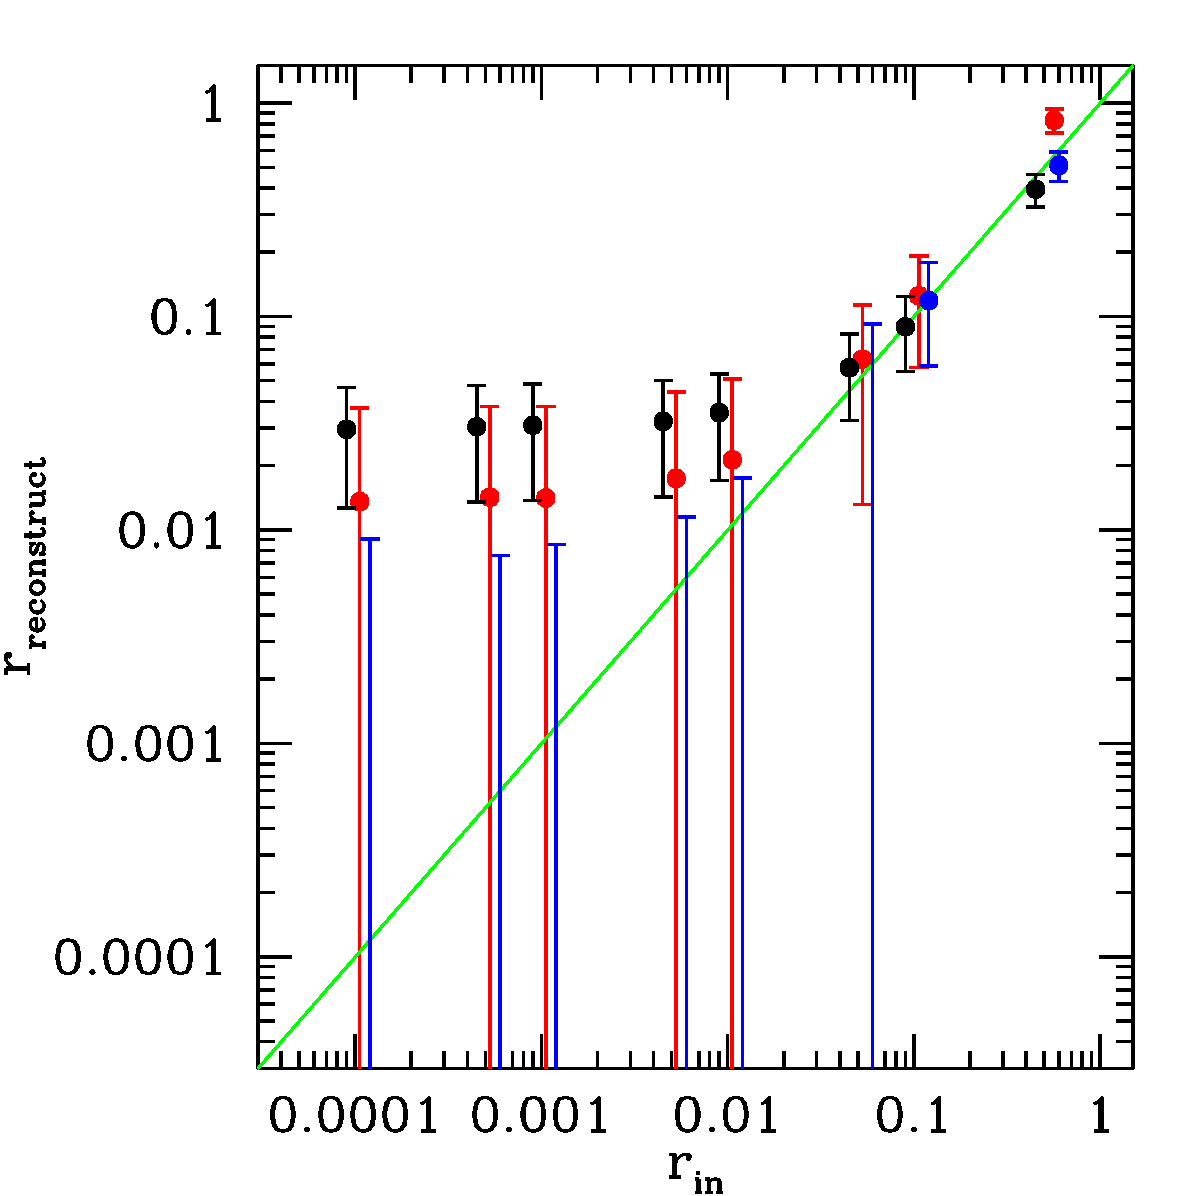
\includegraphics[width=0.45\linewidth]{scanning_rin_rout_planck}
  (b)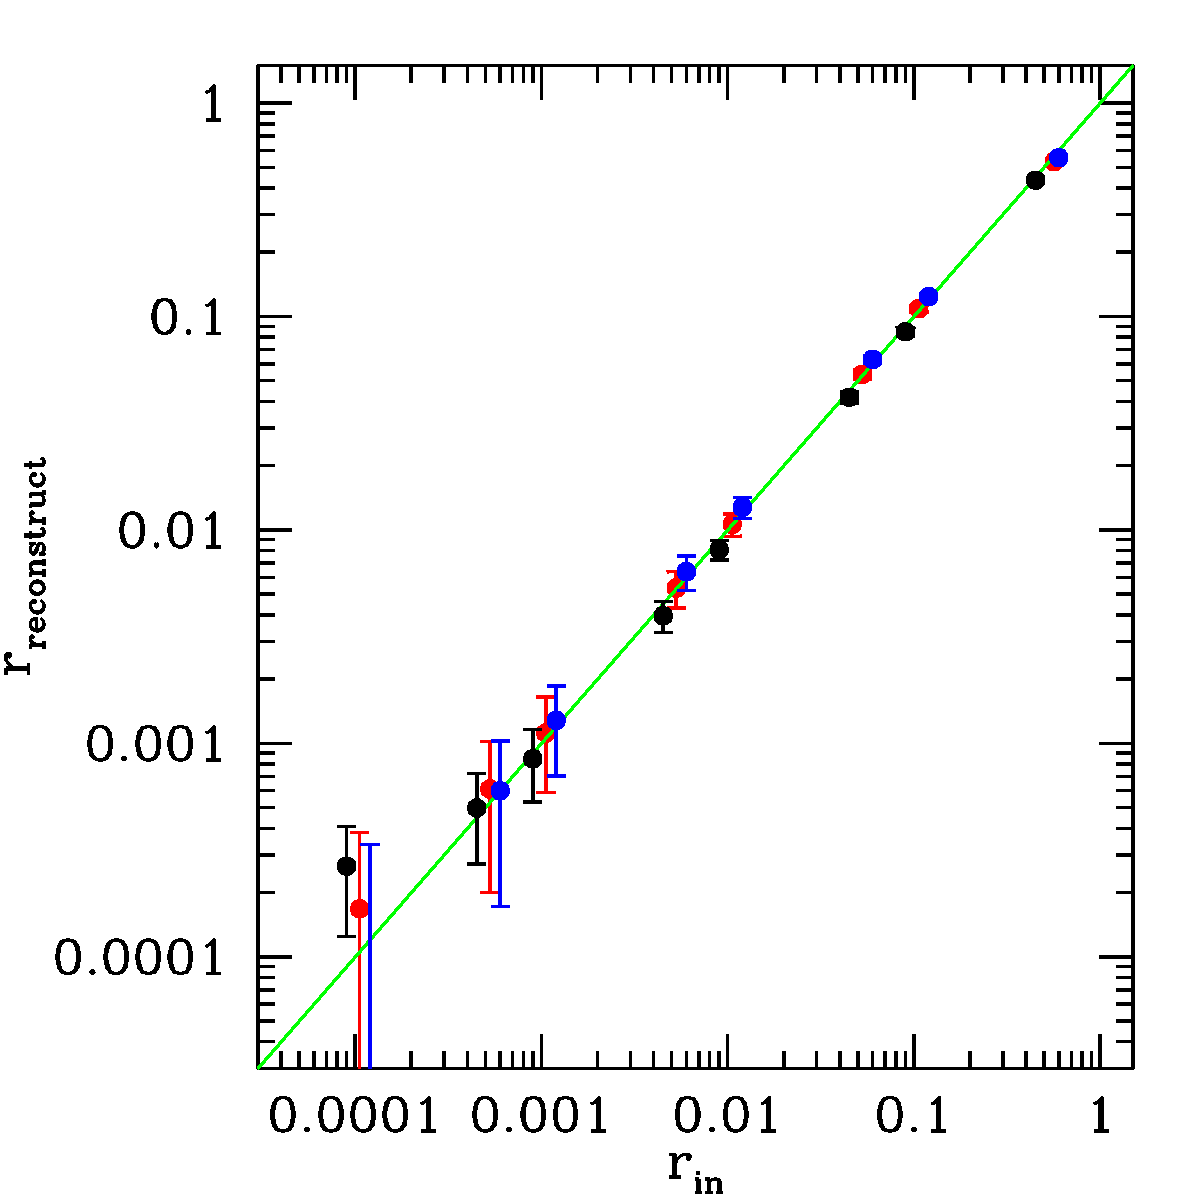
\includegraphics[width=0.45\linewidth]{scanning_rin_rout}

  \caption{The reconstructed values $r_{\mathrm{reconstructed}}$ of
  the input tensor scalar ratio $r_{\mathrm{in}}$ from a (a) Planck
  and (b) CMBPol type experiment with different parameterizations:
  $\pscalar, \ptensor$ (black), the standard parameterization (red),
  $\ln\epsilon$ trajectories (blue). For a Planck type experiment, the
  reconstructed values of $r$ are prior dominated at $r\approx0.05$.}

   \label{fig:rin_rout}
\end{figure*}
\subsubsection{Model selection}
Recently a lot of attention has been devoted to the question of model
selection \cite{Mukherjee:2005wg,Liddle:2006tc}. Given several
competing models with different numbers of parameters, the fundamental
issue is to decide which model describes the data best while at the
same time not introducing ``superfluous'' parameters whose presence is
not warranted by the data. The decision on the usefulness of a
parameter is in part based on the volume of parameter space that one
subjectively deems likely to be allowed. In this work our approach
will be to examine the space of possible inflationary trajectories
without introducing any subjective model selection. Our focus will be
on the effect the increase in the number of parameters will have on
the posterior distribution of the parameters and the implied priors.

\subsection{Searching for nontrivial features in the power spectra}

Although any specific choice of algorithm to generate ``random''
trajectories may be challenged by prior issues as discussed above, we
are interested in methods that can practically detect nontrivial
features in the primordial power spectra. To show that the method we
are advocating in this paper is a viable candidate, we produce mock
data with $\pscalar$ having an ``IR-cascading''
bump \cite{Barnaby2009a, Barnaby2009b}, approximated by
\begin{equation}
P_{\rm bump} = A\left(\frac{k}{k^*}\right)^3e^{-\frac{\pi}{2}\left(k/k^*\right)^2} \ .
\end{equation}
The shape of such a bump can be calculated in the theory, and should be parameterized accordingly in power spectrum reconstruction attempts if we consider
this particular model. Here we examine  whether such a bump is
detectable without knowing the theoretical priori. 

The reconstructed power spectra using monotonic cubic Hermite
interpolation between 11 knots are shown in Figure~\ref{fig:bump}. 
The bump in the scalar spectrum has no effect on the reconstructed tensor spectra, we hence only show scalar trajectories in the plot for a clear view of the details of the reconstructed bump. We notice that the bump is successfully reconstructed. However, the spectrum close to the bump is slightly twisted by the smoothness
assumption (prior) we have chosen. We have also tried natural cubic spline interpolation and varying the number of the knots. We find that the twisting varies with different choices of interpolation method and number of knots, confirming our conjecture that it is a prior-driven effect. 
Despite these prior issues that persist in any trajectory
reconstruction methods, we are able to find the main feature in the power spectrum without knowing the theoretical priori.

\begin{figure}
  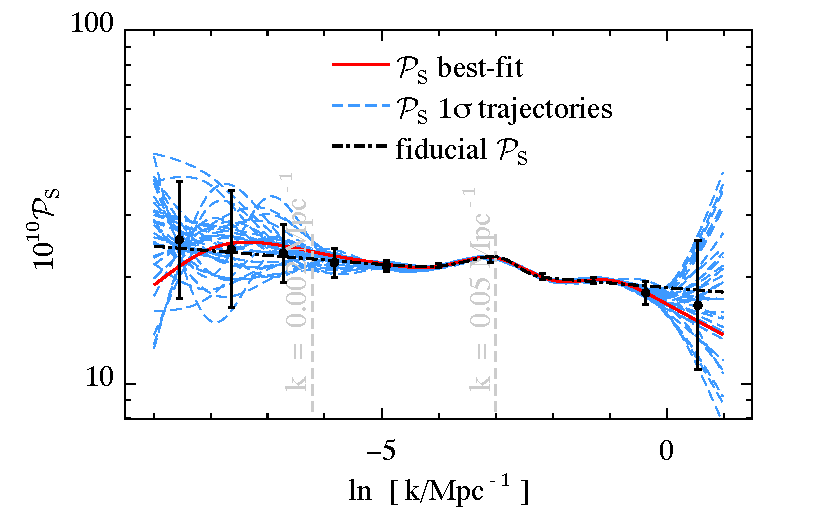
\includegraphics[width=0.9\linewidth]{fc_bump_p11hermite_traj11} 
  \caption{The reconstructed primordial power spectra, using mock data
  with a feature in the scalar power spectrum. A fiducial $r=0$ and
  $n_s=0.97$ model has been used, on top of which an IR-cascading
  bump \cite{Barnaby2009a, Barnaby2009b} with amplitude about 10\% of
  the total $\pscalar$ and with position $k^* = 0.05 \mpc^{-1}$ is
  added to the scalar power spectrum, as shown in dot-dashed black color. Monotonic cubic Hermite
  interpolation is used to interpolate $\ln \pscalar$ between 11 knots.}  
  \label{fig:bump}
\end{figure}



\section{Single field inflation models}\label{sec:single_field}

In this section, we restrict the space of allowed inflationary
possibilities to models driven by single real scalar fields. In this
case, it is straightforward to see that all information about the
inflationary history is encapsulated in the time evolution of the
``slow roll'' parameter $\epsilon$ which we will briefly demonstrate
below.

\subsection{Inflation driven by a single scalar field}
A brief recap of the physics of inflation driven by a single real
scalar field is in order. Assuming the background is given by an FRW
metric
\begin{eqnarray}
  ds^2&=&dt^2-a(t)^2d\vec{x}^2\,,
\end{eqnarray}
with scale factor $a$, and permeated by a homogeneous scalar field
$\phi$ obeying
\begin{eqnarray}\label{eq:scalar_bg}
  \ddot\phi+3H\dot\phi+\partial_\phi V&=&0\,,\\
  \frac{1}{3}\left(\frac{1}{2}\dot\phi^2+V\right)&=&H^2\,,\\
  \frac{1}{2}\dot\phi^2=-\dot H\,,
\end{eqnarray}
where we introduced the Hubble parameter $H=\partial_t \ln a$ and set
the reduced Planck mass to unity $M_p^2\equiv\frac{1}{8\pi
  G}=1$. 

It is well known that small perturbations on top of this homogeneous
background obey
\begin{eqnarray}\label{eq:pert}
  u_k^\pprime + \left(k^2-\frac{z^\pprime}{z}\right)u_k&=&0\,,\\
  v_k^\pprime + \left(k^2-\frac{a^\pprime}{a}\right)v_k&=&0\,,\\
\end{eqnarray}
where $u_k, v_k$ are the perturbations in the scalar and tensor sector
and given by
\begin{eqnarray}
  u_k&=&-\frac{a\dot\phi}{H}\left(\Psi-\frac{H}{\dot\phi}\delta\phi\right)\,,\\
  h_{ij}&=&\int\frac{d^3k}{(2\pi)^{3/2}}\sum_{\lambda=1}^2\frac{1}{a} v_{k,\lambda} e_{ij}(k,\lambda)e^{ikx},
\end{eqnarray}
where $\Psi, h_{ij}$ is the scalar/ tensor part of the metric
perturbation, $e_{ij}$ is the polarization tensor,
$z=\sqrt{2\epsilon}a$, and $f^\prime=a\frac{\partial}{\partial t}f$,
see \cite{Stewart:1993bc} for details.

\subsection{All information is in $\epsilon$}
As mentioned above, all information about the evolution of the
universe, i.e. of the background fields and their perturbations, is
contained in the time evolution of $\epsilon\equiv-\frac{\dot
  H}{H^2}$. This can be seen by rearranging the background equations
(\ref{eq:scalar_bg})
\begin{eqnarray}\label{eq:all_in_eps}
  a&=&e^{-N}\,,\\
  \frac{\partial\phi}{\partial N}&=&\pm\sqrt{2\epsilon}\,,\\
  \frac{\partial \ln H}{\partial N}&=& - \epsilon\,,\\
  V&=&H^2(3-\epsilon)\,,
\end{eqnarray}
where $dN=-Hdt$ is the number of e-folds, so that there is a mapping
from a given expansion history $\epsilon(t)$ plus an integration
constant for $H$ to a scalar field potential that allows for such a
$\epsilon$ trajectory. Note that the integration constant for $\phi$
is irrelevant as this corresponds to a constant shift of the
potential, whereas the sign ambiguity is due to the fact that sending
$\phi\rightarrow -\phi$ does not change the physics either.

Most importantly, for a given energy scale $H(k_{\rm pivot})$,
$\epsilon(t)$ is all that is needed to plug into the perturbation
equations (\ref{eq:pert}), so that knowledge of $\epsilon$ also
completely determines the knowledge of the perturbation spectra.

It should also be noted that instead of providing $\epsilon$ as a
function of some time variable, it is equally viable to provide it as
a function of the (comoving) wavenumber $k$, making use of the fact
that inflationary perturbations of wavenumber $k$ freeze out around
the time when $k\lesssim aH$ (although see \cite{Vaudrevange:2009ag} for an
inflationary model in which perturbations do not freeze out).

In short, having full knowledge of
$\epsilon(k)\equiv \epsilon\vert_{k=\ln(aH)}$ trajectories, it is
straightforward to compute the scalar potential as well as the
behavior of the scalar and vector perturbations.

\subsection{The $\epsilon$ trajectory and different priors}

Working with $\epsilon$ as a trajectory has another advantage: it is
well known that the inflationary condition $\ddot a>0$ is equivalent
to
\begin{eqnarray}
  \ddot a&\equiv& a(\dot H+H^2)=aH^2(1-\epsilon)\stackrel{!}{>}0\,.
\end{eqnarray}
In other words, $\epsilon<1$ during a period of accelerated
expansion. On the other hand, for an expanding universe
$\epsilon\equiv-\frac{\dot{H}}{H^2}>0$ as $\dot H<0$. Thus, $\epsilon$
trajectories during inflation are required to lie between
\begin{eqnarray}
  0<\epsilon<1\,.
\end{eqnarray}

It should be noted that this ``inflationary prior'' is not realized by
the usual approach to model building. Writing down models for single
field inflation usually means writing down a potential for $\phi$
(possibly as a power series). This does not give a uniform prior for
$\epsilon$ between $[0,1]$, but rather a strong preference for ``slow
roll'' models, that is, models with $\epsilon\ll1$ and $\vert
d\ln\epsilon/d\ln k\vert\ll 1$. While this is a valid subjective
choice of prior, it seems an interesting questions as to what the data
prefers if we do not employ this slow roll prior. In particular, the
condition $\vert d\ln\epsilon/d\ln k\vert\ll 1$ can be relaxed to some
extent without spoiling a nearly scale invariant scalar power
spectrum.

Unfortunately, it turns out that using straight $\epsilon(\ln k)$
trajectory functions introduces spurious detections of tensors which
are purely prior driven: even though the values of the trajectory
function at the knots are chosen uniformly between $[0,1]$, the
interpolation leads to a systematic bias against small values of
$\epsilon$, see Appendix~\ref{app:interpolation_issues}. Hence we need
to slightly change the trajectory function.

Most interest lies in the spectra index
$n_s-1\approx-2\epsilon-d\ln\epsilon/d\ln k$ (which is also well
constrained by data). In the case that $\epsilon$ is small, the
deviation from scale-invariance of the scalar power spectrum is due to
the term $\frac{d\ln\epsilon}{d\ln k}$. This makes it a suitable
choice of trajectory function. However, it slightly complicates the
step of verifying that the trajectory corresponds to an inflating
universe, but avoids the purely prior driven detection of tensors.

Figure~\ref{fig:p7eps} shows the reconstructed power spectra when
using a $7$ knot cubic Hermite polynomial expansion of
$\frac{d\epsilon}{d\ln k}$. The best-fit trajectories are shown in
solid red, whereas the trajectories from the $1\sigma$ interval are
plotted in solid blue. Even though there are some features in
$\mc{P}_S$ (Figure~\ref{fig:p7eps}a), the corresponding
$C_{\ell}^{TT}$ spectra (Figure~\ref{fig:p7eps}b) agree very well with
observations. 

As can be seen in Figure~\ref{fig:p7eps_potentials}(a), the underlying
$\epsilon$ trajectories are relatively smooth within the interval $\ln
\frac{k}{\mpc^{-1}}=-5\dots0$. On larger scales, there are some wild
excursions with $\epsilon$ even becoming non-monotonic. Yet the
overall smoothness of the $\epsilon$ trajectory is quite striking,
given the fact that the extrapolation used $7$ knots -- a relatively
large number. For comparison, the unconstrained $\pscalar, \ptensor$
expansion of the previous section contained much wilder trajectories
when using $7$ knots for $\pscalar$.

\begin{figure*}
\centering
  %\begin{tabular}{ll}
  \hskip -0.4\in
    \begin{minipage}{0.58\linewidth}
      (a)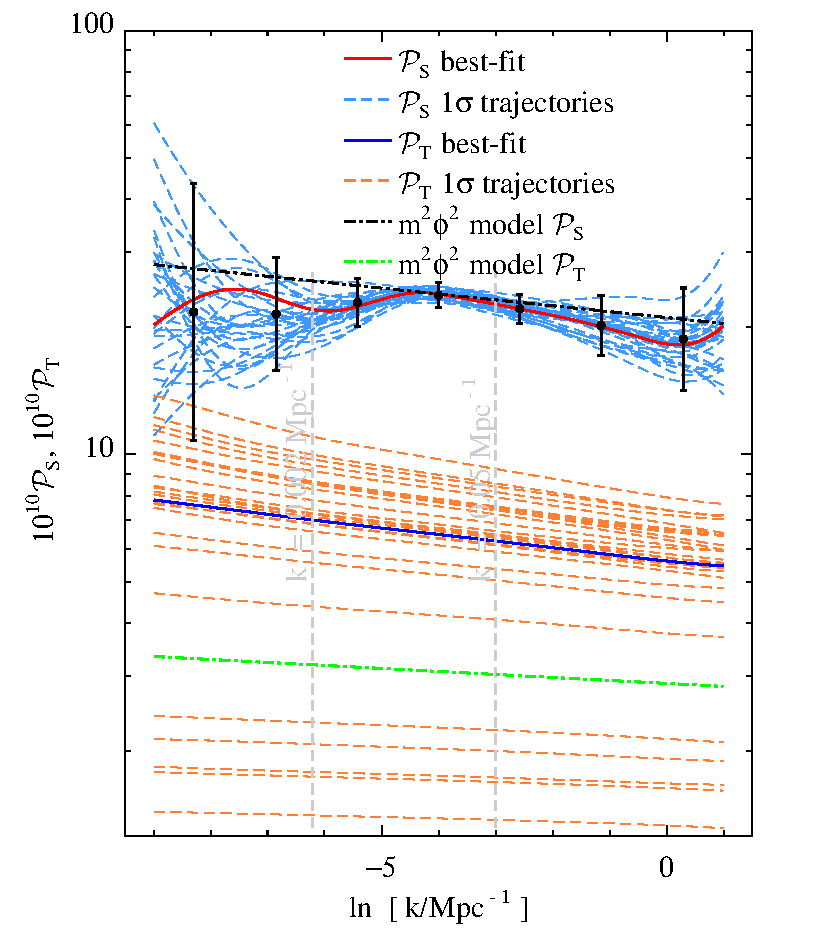
\includegraphics[width=0.9\linewidth]{p7eps_traj11}%
    \end{minipage}
   \begin{minipage}{0.3\linewidth}
      (b)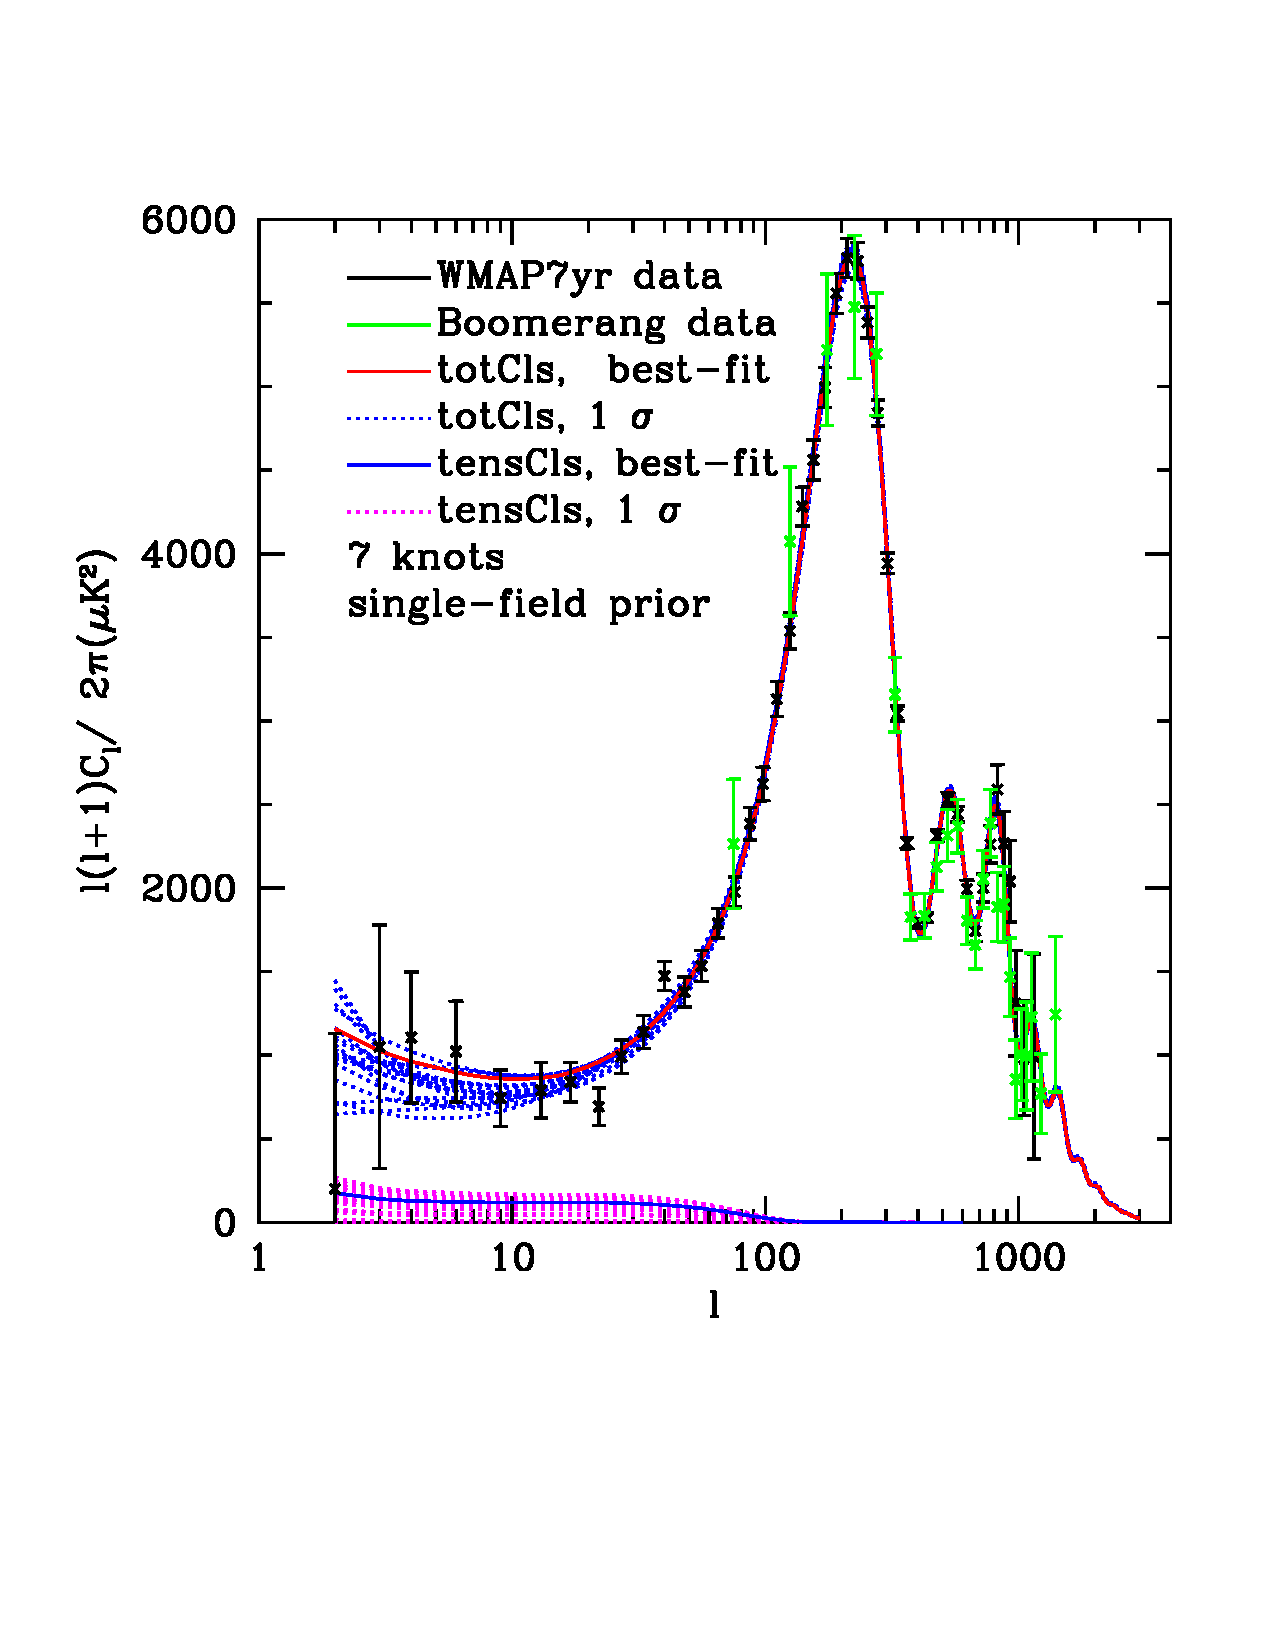
\includegraphics[width=0.9\linewidth]{p7eps_TT} \\
      (c)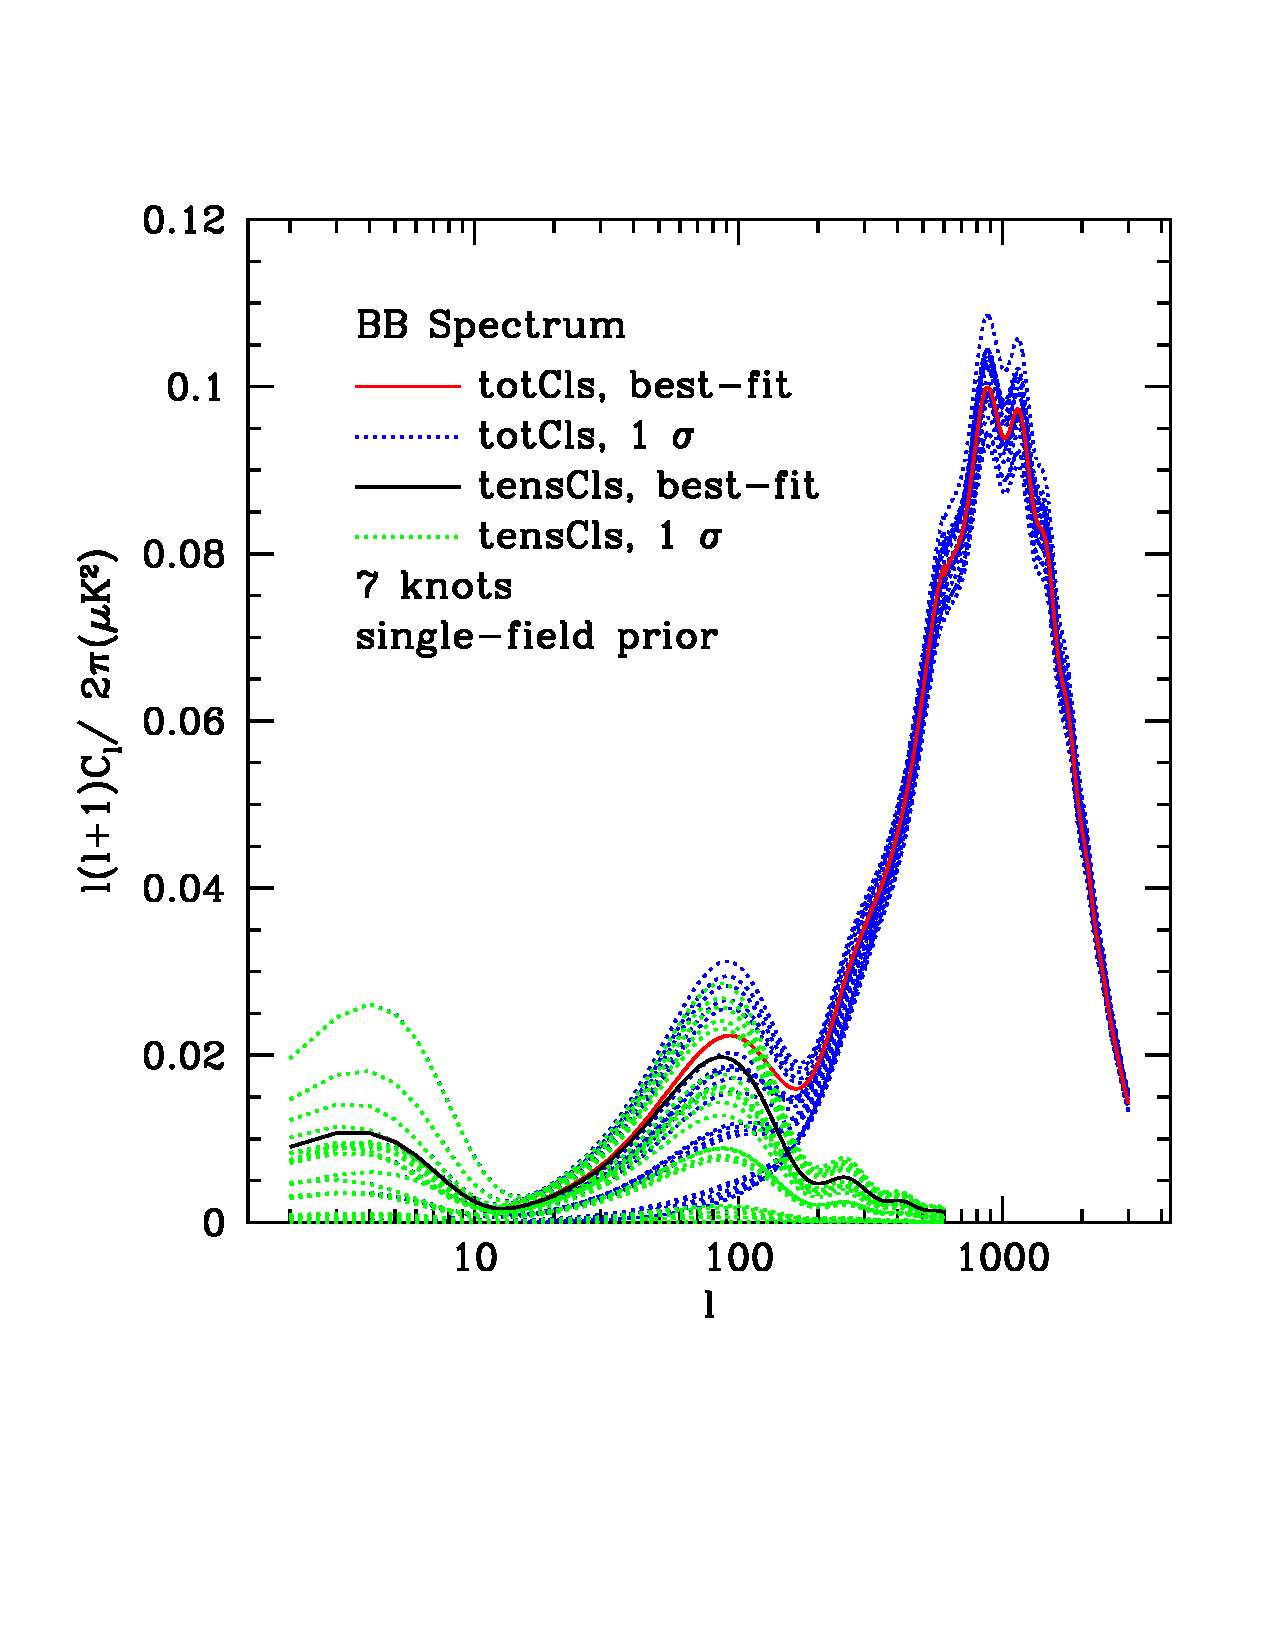
\includegraphics[width=0.9\linewidth]{p7eps_BB} 
    \end{minipage}
  %\end{tabular}
  \caption{(a)Reconstructed power spectra when using a $7$ knots
    expansion of the $\frac{d \epsilon}{d\ln k}$ trajectory. (b) TT
    angular power spectrum (c) BB angular power spectrum. Same color
    scheme as in Figures~\ref{fig:7knot_Ps_Pt}, \ref{fig:7knot_Cl_TT_BB}}
  \label{fig:p7eps}
\end{figure*}


\subsection{Reconstructing the potential}

As mentioned above, all information about single field inflation is
contained in the $\epsilon$ trajectory. In particular, we can
reconstruct the shape of the scalar field potential $V(\phi)$ from
knowledge of the (time) evolution of $\epsilon$.

This is most readily achieved by rewriting Eq.~(\ref{eq:all_in_eps})
as
\begin{eqnarray}
  V(\ln k)&=&H^2(\ln k)\left(3-\epsilon(\ln k)\right)\,,\\
  \frac{\partial \phi}{\partial \ln k}&=&\pm\frac{\sqrt{2\epsilon(\ln k)}}{1-\epsilon(\ln k)}\,,\\
  \frac{\partial \ln H}{\partial \ln k}&=& - \frac{\epsilon(\ln k)}{1-\epsilon(\ln k)}\,.
\end{eqnarray}
This allows us to map the reconstructed $\epsilon$ trajectories from
Figure~\ref{fig:p7eps_potentials}(a) to the potential $V(\phi)$, see
Figure~\ref{fig:p7eps_potentials}(b). The red line represents the best
fit potential, whereas the blue lines are drawn from the $1\sigma$
interval around the best fit. Note that both the potential has been
rescaled and the field values shifted so that the differences in shape
become more apparent.
\begin{figure*}
  (a)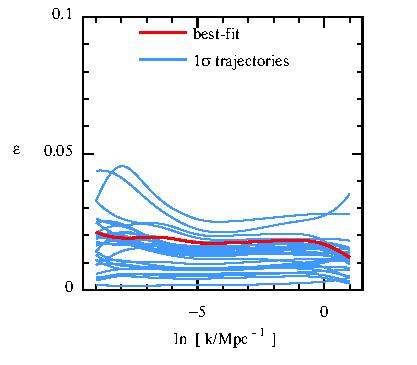
\includegraphics[width=0.45\linewidth]{p7eps_traj2}
  (b)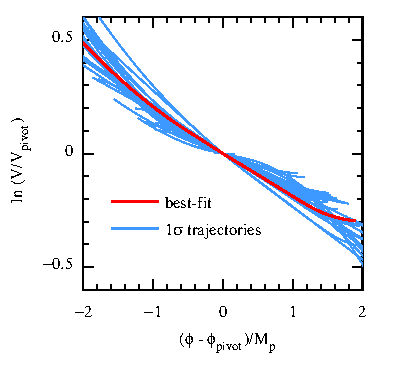
\includegraphics[width=0.45\linewidth]{p7eps_traj1}
  \caption{(a) $\epsilon$ trajectory using an order $7$ knots, natural
    monotonic cubic Hermite interpolation of the $\epsilon$ trajectory
    and (b) Reconstructed potentials. The best fit trajectories are
    shown in red, and the ones drawn from the $1\sigma$ interval
    around it in blue.}
  \label{fig:p7eps_potentials}
\end{figure*}


Just as with the independent tensor and scalar spectra about, we shall
now briefly discuss the performance of using $\epsilon$ trajectories
with forecast data. We examine the same two fiducial models as
in Section~\ref{sec:7knots}.
\begin{figure*}
  (a)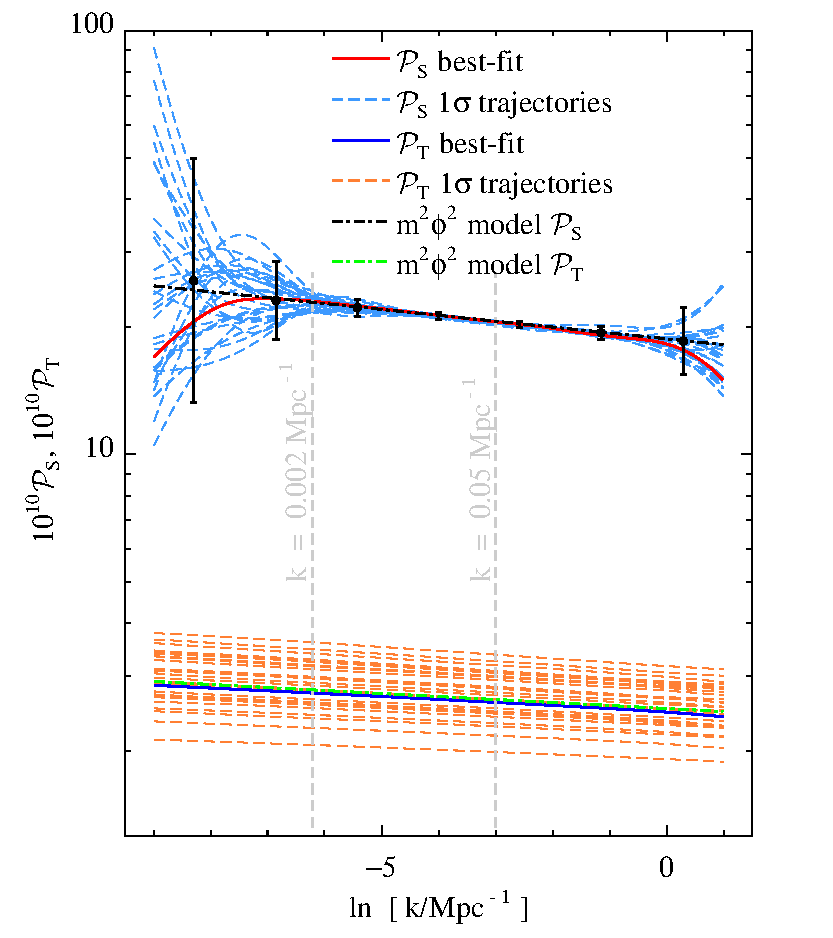
\includegraphics[width=0.45\linewidth]{fc_p7eps_traj11}
  (b)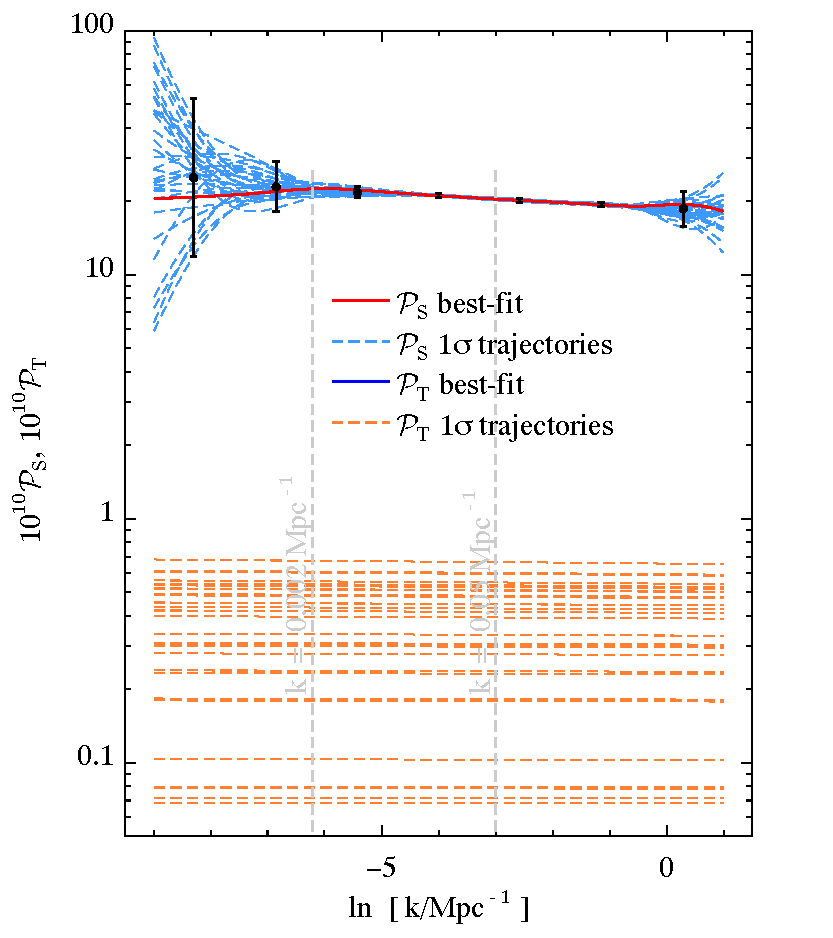
\includegraphics[width=0.45\linewidth]{fc_p7eps_r0_traj11}
  \caption{(a) Forecast for $m^2\phi^2$ inflation with $r=0.13$,
    $n_s=0.97$ (b) Forecast for single field inflation with $r=0$.}
  \label{fig:mock_eps}
\end{figure*}

For the fiducial $V(\phi)=m^2\phi^2$ model with $r=0.13$,
Figure~\ref{fig:mock_eps} shows that using the $\epsilon$
trajectories, both the scalars and tensors are reconstructed with high
precision. The reason for this improvement in performance over the
independent $\pscalar$, $\ptensor$ trajectories is the additional
theoretical information we added to the picture: the fact that scalars
and tensors obey the consistency condition $n_t=-\frac{r}{8}$. In this
framework, a well constrained scalar spectrum will automatically
induce small error bars on the tensors.


\section{Summary and Conclusions}\label{sec:conclusions}
In this paper we study different ways to scan over inflationary models
in order to explore the range of primordial power spectra that can be
generated. We investigate the inverse problem of how to reconstruct
the primordial power spectra of scalar and tensor perturbations from
observational data.

While most of the previous studies on the ensemble of inflationary
models used a diversity of potential functions $V(\phi)$, we focus
instead on the trajectory functions, as described by the evolution of
$\pscalar$, $\ptensor$ or $\epsilon$ during inflation.

If the time flow along of the inflationary trajectory is measured in
terms of number of $e$-foldings $N$, the minimum duration of inflation
$\Delta N$ generally depends on the inflationary model. The time
interval during which the inflationary trajectories are examined can
be made precisely independent of the model if time is measured in
comoving momenta of fluctuations $\ln k$ provided one assumes that
inflation does not proceed in staggered phases. Thus we are dealing
with an ensemble of trajectory functions over a fixed domain of the
argument which can be conveniently expanded in various function bases
such as Chebyshev polynomials or B-splines, providing both optimal
approximation and numerically fast routines for evaluation and taking
derivatives.

We demonstrate explicitly how the traditional parameterization using
$A_s, n_s, n_{\mathrm{run}}, r$ is exactly equivalent to a specific
trajectory approach and show that the parameters reconstructed by both
parameterizations are in very good agreement. As a further test of
reliability, we show that simulated spectra smeared by Planck errors
can be reconstructed with $\pscalar, \ptensor$ as well as
$\epsilon$ trajectories -- albeit with some residual uncertainty
pertaining to the shape of the (implicit) prior distributions.

In contrast to existing methods like the flow equations, the scanning
inflation approach as presented here does not involve any integration
of differential equations, making it numerically extremely fast. The
trajectory choice of $\pscalar, \ptensor$ does not respect the
consistency relation connecting them in the case of inflation driven
by a scalar field. Of particular importance, we have shown that
nontrivial features in the scalar power spectrum can be detected
without using theoretical prior knowledge about the shape of the
feature.

Incorporating the consistency relation naturally leads to taking
another choice for the trajectory function, the deceleration parameter
$\epsilon$, where it becomes necessary to perform a single integration
to obtain the Hubble trajectory needed to compute the power
spectra. In this case, one can describe all inflationary dynamics
(both of the background and the perturbations) in terms of the
evolution of e.g. $\epsilon(\ln k)$, also reconstructing the shape of
the potential of the scalar field driving inflation.

We identified the importance of priors and the ways their bias can
change the outcome of MCMC parameter estimation. Even though
parameters are sampled with flat priors, the prior distribution of the
power spectra can be implicitly altered, a fact that is easy to
overlook. Exploring various choices of priors, we demonstrated that it
is possible to at least partially smooth the inhomogeneity of the
priors, making the distribution uniform and only slightly depending on
the position in $k$-space.

Implied priors most significantly impact the value of the tensor
scalar ratio $r$. Using a uniform and homogeneous prior on
$\ln\pscalar, \ptensor $ in an expansion to order $(3,1)$ --
i.e. a constant tensor spectrum --, the upper limit on
$r<0.33(95\%{\rm CL})$ is compatible with the limit $r<0.36(95\%{\rm CL})$
obtained using the standard parameterization given the fact that the
parameters trajectory parameterization are non-linear combinations of
the standard parameters. 

Let us finish with a final remark on the maximum amount of complexity
that can be present in inflationary trajectories. In principle, one
can increase the expansion order to arbitrarily high numbers, allowing
for more and more structure in the trajectories. Here we
conjecture\footnote{We thank Andrei Linde for useful discussions of
this point.} that there is a natural limitation on the structure and
fine details of the trajectories, namely that the details associated
with features on time scales smaller than the inverse Hubble scale
$H^{-1}$ are irrelevant. This is to say only those features on a scale
exceeding one $e$-folding are relevant. There are numerous examples in
the literature with the calculations of the spectra from inflation
with various features like breaks in the potentials, marginal
inflation etc. All of them show that the features of the corresponding
power spectra are smooth on scales less than $H$. Heuristically it can
be understood by analogy with diffraction patterns in wave optics,
where in our case the wavelength of interest is $H^{-1}$.

This conjecture implies that in order to exhaust all potential
inflationary trajectories describing the physics in the $k$-range
accessible to observations -- i.e. about $10$ $e$-folds -- it is
sufficient to consider trajectories only up to order $10$, making
inflation a science of only $10$ numbers.


\section*{Acknowledgments}
All computations were performed on thecomputing clusters at CITA. We gratefully acknowledge financial support by
NSERC, CIFAR and CFI.

\appendix
\section{Various function bases}\label{app:polynomials}
The current observational data explore about ten e-folds of comoving
wave-length, roughly corresponding to the interval
$-9<\ln{\left(k/\Mpcinv\right)}<1$. Let us define this interval as
``observable interval''. The spectra on scales outside the observable
interval do not have essential impact on the cosmic observables. Any
reasonable extrapolation will do as good. We simply use constant
$\pscalar$ for these extra-large and extra-small scales. Natural cubic
spline interpolation is our default option to interpolate
$\ln\pscalar$ within the observable interval. Alternative
interpolation methods are Chebyshev interpolation and monotonic cubic
Hermite interpolation. The Chebyshev interpolation defines a unique
$n-1$-th order polynomial passing the $n$ given points at the
knots. Both natural cubic spline interpolation and monotonic cubic
Hermite interpolation assume third order polynomial between two
neighbor knots. Natural cubic spline defines a unique interpolated
curve by matching the second order derivatives across the knots, with
an additional assumption that the second order derivative vanishes at
the two boundaries. The cubic Hermite interpolation only requires the
first order derivative to be continuous across the knots. The extra
$n$ degrees of freedom is fixed by choosing the first order derivative
at the $i$-th knot. For generic cubic Hermite interpolation where the
piecewise monotonicity is not required, the derivatives can be chosen
as

\begin{equation}
\Delta_i \equiv \left\{
\begin{array}{ll}
\left[f(x_{2}) - f(x_{1})\right]/(x_{2}-x_{1}) & \text{, if } i = 1 \\
\left[f(x_{n}) - f(x_{n-1})\right]/(x_{n}-x_{n-1}) & \text{, if } i = n \\
\left[f(x_{i+1}) - f(x_{i-1})\right]/(x_{i+1}-x_{i-1}) & \text{, else}
\end{array}
\right.
\end{equation}

where $x_i$ is the $i$-th knot. For monotonic cubic Hermite
interpolation, the piecewise monotonicity of $f(x)$ between two
neighbor knots is achieved by further adjusting $\Delta_i$. First, for
$i=1,2,...,n-1$, if $f(x_i)=f(x_{i+1})$, set
$\Delta_i=\Delta_{i+1}=0$. Second, for $i=1,2,...,n-1$ where
$f(x_i)\ne f(x_{i+1})$, define
$\alpha_i=\Delta_i(x_{i+1}-x_i)/\left[f(x_{i+1})-f(x_i)\right]$ and
$\beta_i = \Delta_{i+1}(x_{i+1}-x_i)/\left[f(x_{i+1})-f(x_i)\right]$;
If $\alpha_i^2+\beta_i^2>9$, update $\Delta_i$ and $\Delta_{i+1}$ to
be $3\alpha_i\Delta_i/\sqrt{\alpha_i^2+\beta_i^2} $ and
$3\beta_i\Delta_{i+1}/\sqrt{\alpha_i^2+\beta_i^2}$, respectively.


To summarize, the parameterization is:
\begin{enumerate}
\item Flat prior on $\ln\pscalar$, if $k$ is a knot. 
\item Interpolate $\ln \pscalar (\ln k)$, if $-9<\ln\left(k/\Mpcinv\right)<1$ and $k$ is not a knot.
\item Extrapolation: $\ln \pscalar(\ln k)  =\cond[\ln \pscalar][\ln\left(k/\Mpcinv\right)=-9]$ , if $\ln\left(k/\Mpcinv\right)<-9$;
$\ln \pscalar(\ln k)  =\cond[\ln \pscalar][\ln\left(k/\Mpcinv\right)=1]$, if $\ln\left(k/\Mpcinv\right)>1$.
\end{enumerate}

Uniformly distributed knots from $\ln (k/\Mpcinv) = -9$ to $\ln
(k/\Mpcinv) =1$ are used for natural cubic spline interpolation and
monotonic cubic Hermite interpolation. For Chebyshev interpolation we
choose the nodal points of Chebyshev polynomials, i.e., the $n$
solutions of $n$-th order Chebyshev polynomial $T_n(x)=0$, with
$x\equiv \frac{\ln (k/\Mpcinv) + 4}{5}$. The Chebyshev polynomials
along with the particular pattern of knots are used for better fitting
and numerical stability \cite{CPB}.


\section{Implicit Priors of Random Trajectories}\label{app:interpolation_issues}

In this appendix we examine the priors that are implicit in the choice
of trajectory function and their impact on parameter estimation via
Markov Chain Monte Carlo (MCMC) algorithms in detail.

Traditionally assuming inflation driven by a scalar field, the prior
for inflationary models is that $V(\phi)$ is sufficiently flat and
smooth such that the primordial power spectra are only mildly broken
scale invariant and can be parameterized by $(n_s, n_{\mathrm{run}},
r)$. Ignoring this theoretical bias, the interpolating functions in
the scanning approach will allow for radically broken scale
invariance. Using different trajectory functions and expansion bases,
we shall investigate the shape of the implied priors on the
traditional parameters.

We generate an ensemble of spectral trajectories $\ptensor$ using
the methods based on the Chebyshev decomposition described in
Section~\ref{sec:spectral_trajectories} and demonstrate how the
positivity requirement for $\ptensor$ influences the prior.

The function $\ptensor$ must be positive $\ptensor>0$ with a negative
slope $\frac{d \ptensor}{d\ln k}<0$ because Hubble is a decreasing
function of time. This implies that even though the values of
$\ptensor$ at the nodal points are sampled with a uniform prior, the
prior distribution of $\ptensor$ on and especially in between nodal
points is rather complex and peaked at a value larger than zero, see
Figure~\ref{fig:prior_distribution}.
\begin{figure*}
  %reindeer:~/projects/scanning.falcon/Chebyshev/PR5_PG5_non_monotonic
  %reindeer:~/projects/scanning.falcon/Chebyshev/PR5_PG5
  (a)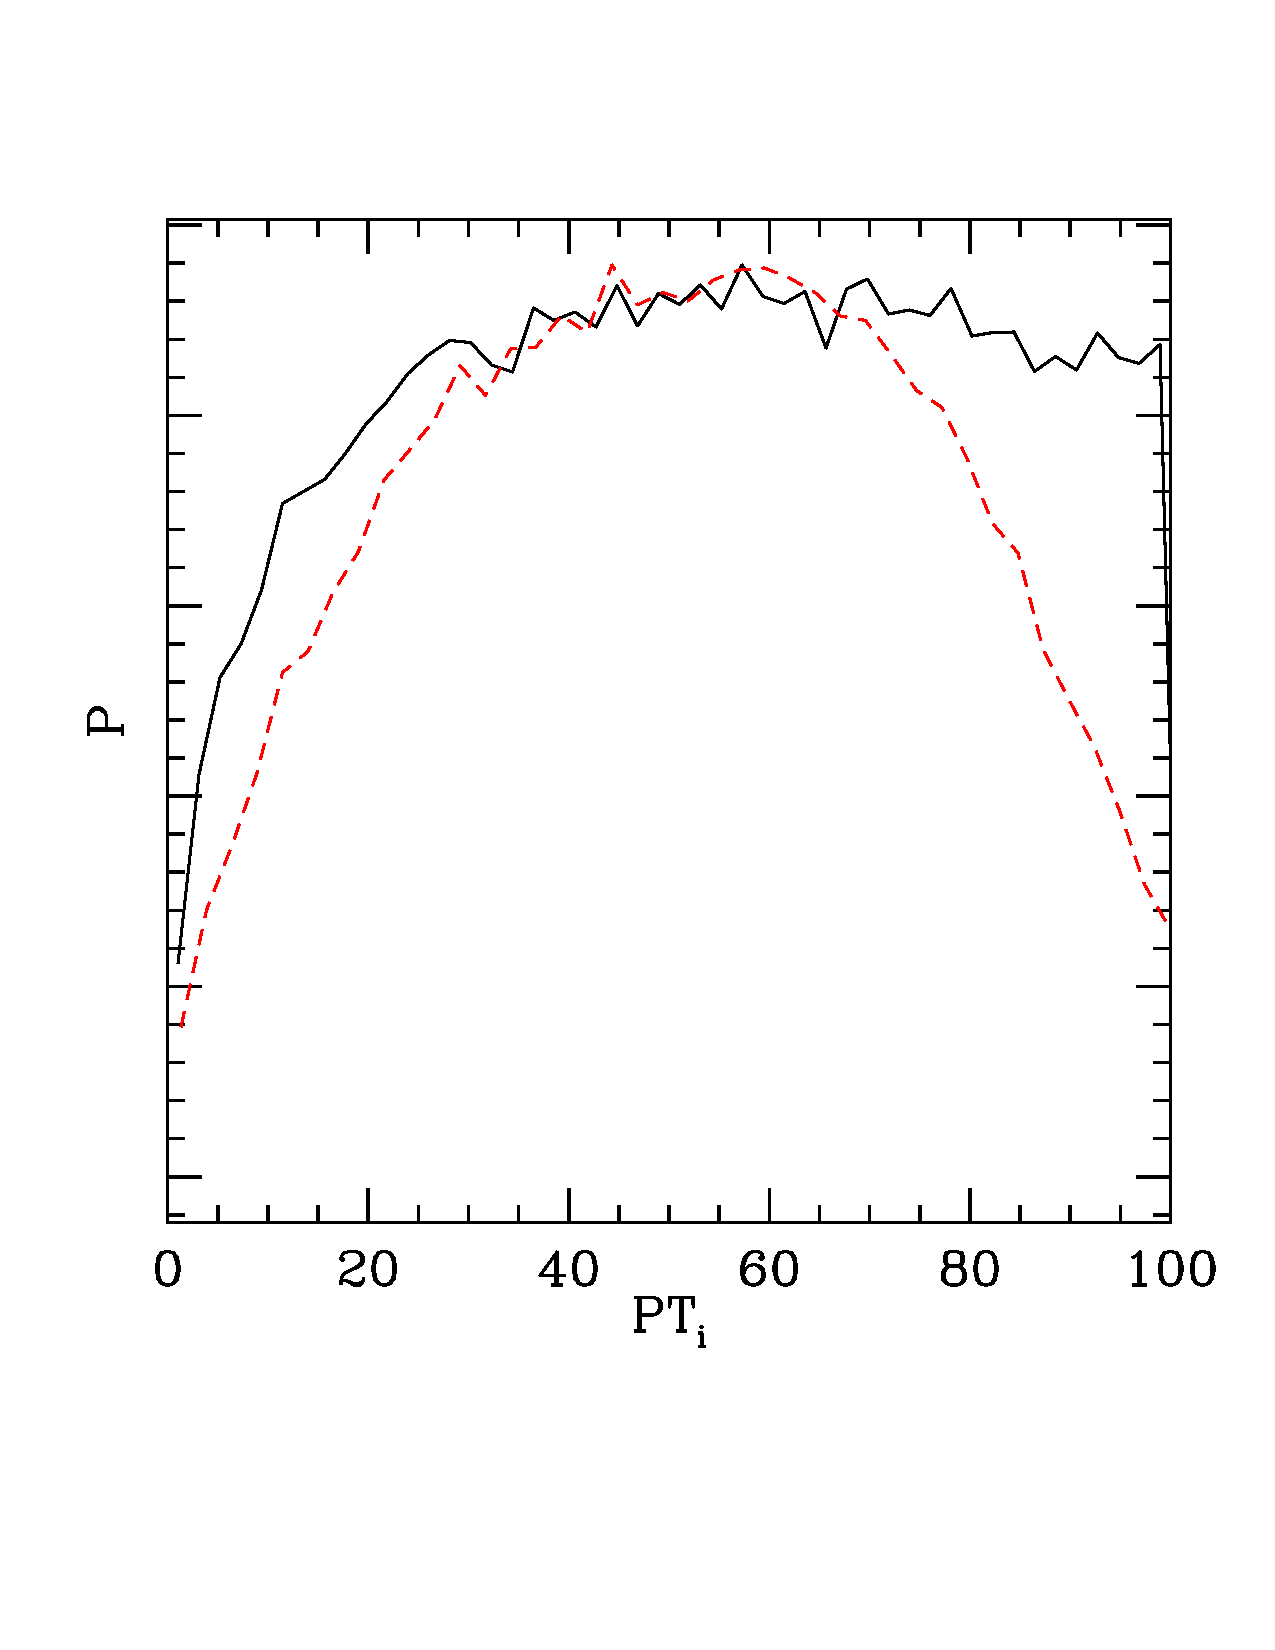
\includegraphics[width=0.45\textwidth]{PR5_PG5_non_monotonic_PG_prior}
  (b)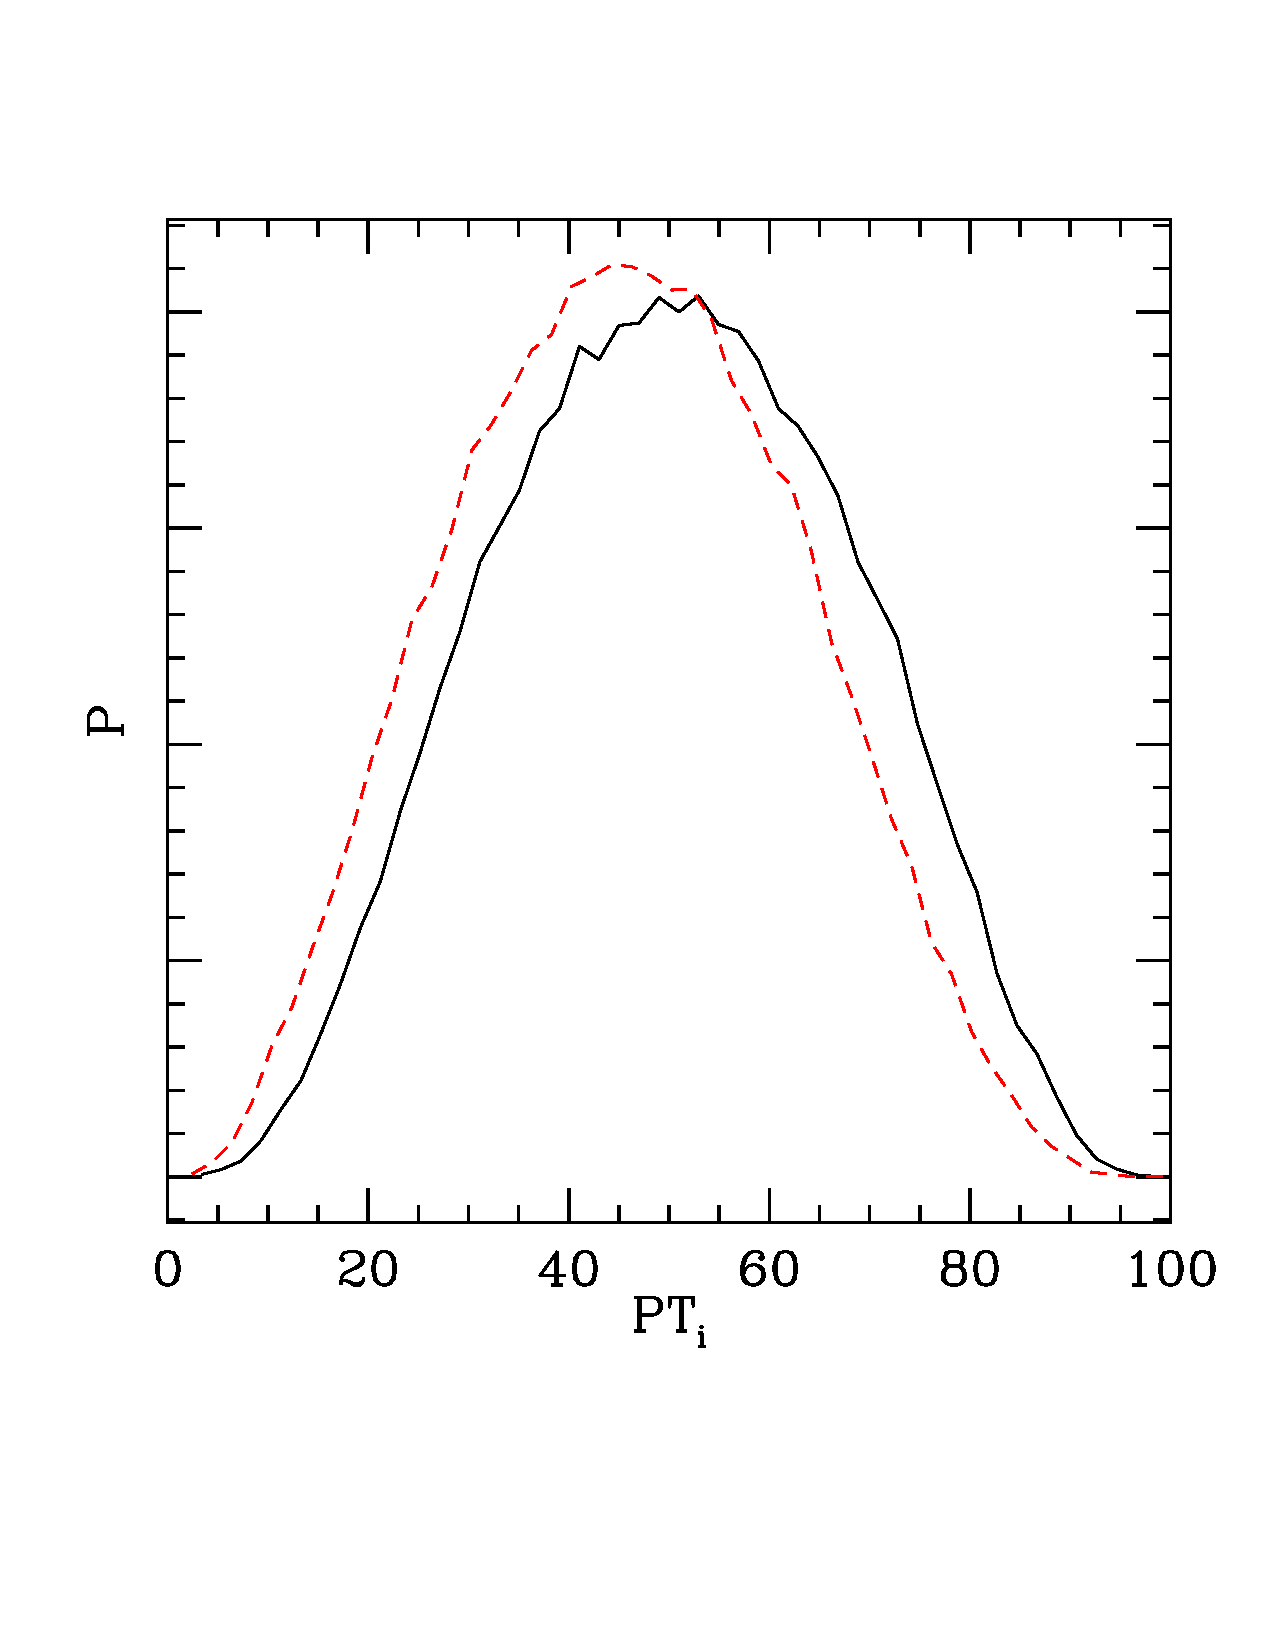
\includegraphics[width=0.45\textwidth]{PR5_PG5_PG_prior}
  \caption[Prior distribution for monotonic and non-monotonic tensor
    power spectra]{The prior probability distribution of a Chebyshev
    interpolation of $\ptensor$ to order $5$ at the third nodal
    point (black solid curves) and in between nodal points (red dashed
    curves) for (a)non monotonic and (b) monotonic
    $\ptensor$. The fall-off of the distribution at lower values
    of $\ptensor$ even on the nodal point is due to the fact that
    non-physical trajectories, i.e. those with $\ptensor<0$, are
    rejected. Therefore if the values at the third nodal point is
    close to zero, trajectories can potentially dip below zero and
    therefore will be discarded. In between nodal points,
    interpolation effects cause the distribution to be peaked. In the
    monotonic case, even at the nodal points enforcing monotonicity
    makes the distribution fall off at high values of $\ptensor$,
    so that the distribution is peaked even at the nodal points, and
    the only effect of moving away from the nodal points is a slight
    shift in the position of the peak.}
  \label{fig:prior_distribution}
\end{figure*}
Panel (a) of this figure shows the prior probability distribution of a
non monotonic Chebyshev interpolation of $\ptensor$ to order $5$
at the third nodal point (black solid curve) and in between nodal
points (red dashed curve). At the nodal point, the distribution should
ideally be flat, however due to the positivity of $\ptensor$ the
probability distribution falls off towards lower values of
$\ptensor$. In between nodal points, an interpolation effect is
responsible for the peak of the probability distribution:

Naively one might expect that sampling uniformly a trajectory function
at a number of nodal points in $\ln k$ and interpolating would also
lead to a more or less uniform distribution of function values in
between the sampled points. But this is only true for functions which
do not have to fulfill any constraints. In case there are any
restrictions on the functions, e.g. enforcing positivity of
$\pscalar, \ptensor$, or restricting them to a finite range,
the prior will generally depend on the location in $k$-space, changing
the picture dramatically. In case of constrained trajectory functions,
the prior distribution becomes peaked away from zero despite being
flat at nodal points. This can be understood in terms of a simple
frequentist argument for example in a linear interpolation between two
points $(A, y(A)), (B, y(B))$, denoted by the red dots in
Figure~\ref{fig:linear_prior}a. The vertical position of both points is
chosen with a uniform prior $P(A)=P(B)=1$, $(y(A),y(B)) \in [0,1]$.
For the value of $y(C)$ to be zero, both $y(A)$ and $y(B)$ have to be
zero, whereas for say $y(C)=0.5$, the pair $(y(A), y(B))$ can have
values $(1.0,0.0), (0.999,0.001),\dots$, therefore it is much more
likely for $y(C)$ to be $0.5$ than to be zero.

Performing a more quantitative analysis of the situation, it is
straightforward to calculate the prior distribution of the point
$y(C)$ which is located in the midpoint between $A$ and $B$,
\begin{eqnarray}
  P(C)&=&\int_0^1\!d A\, \int_0^1\!d B\, P(A) P(B)\, \nonumber\\
  &&\phantom{bla}\times\delta\left(C-(A+(B-A)/2)\right) \nonumber\\
  &=&\left\{\begin{array}{ll}4(1-C), & \frac{1}{2}<C\le1\\4C,& 0\le C\le\frac{1}{2}\end{array}\right.\, ,\, 
\end{eqnarray}
to be shaped like a triangle, see Figure~\ref{fig:linear_prior}(b).
\begin{figure*}
  \begin{center}
    %reindeer:~/projects/scanning/doc/paper2007/fig_linear_prior.sm
    (a)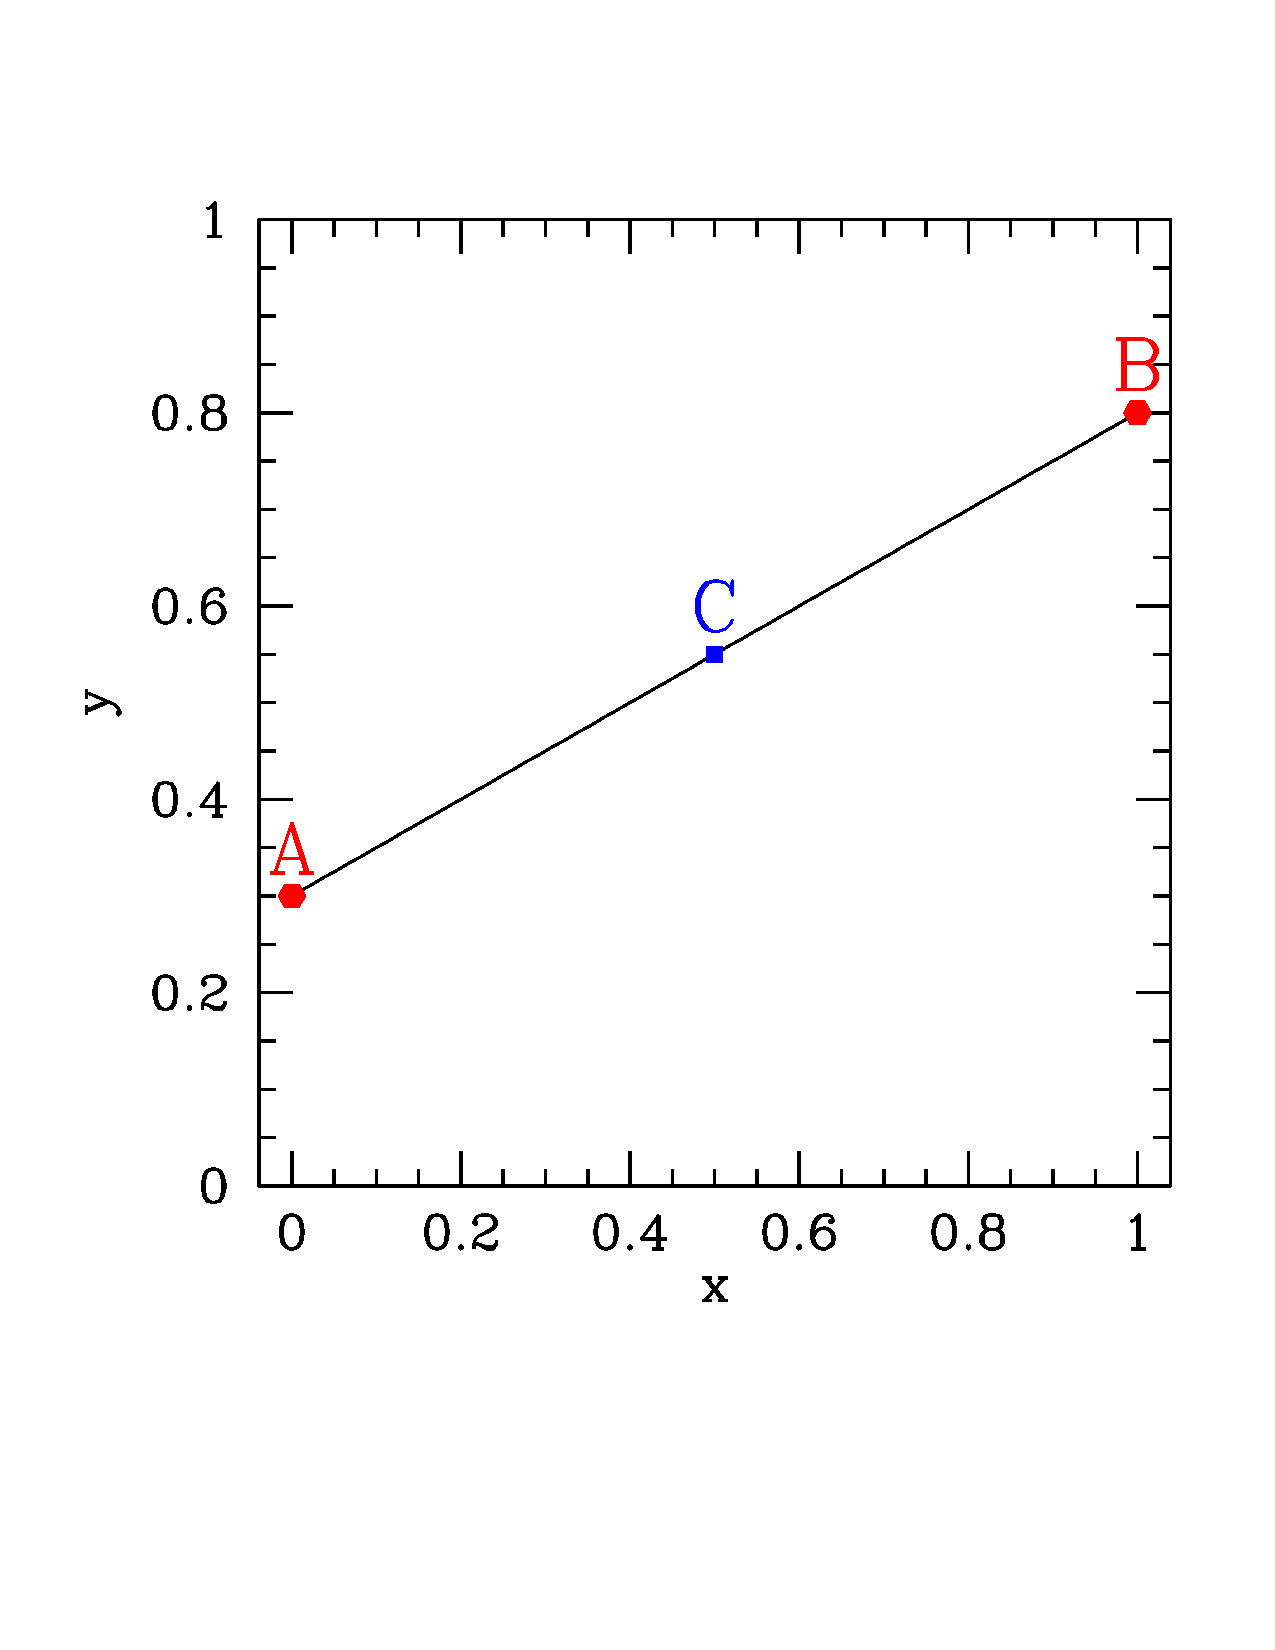
\includegraphics[width=0.45\textwidth]{fig_linear_prior_a}
    (b)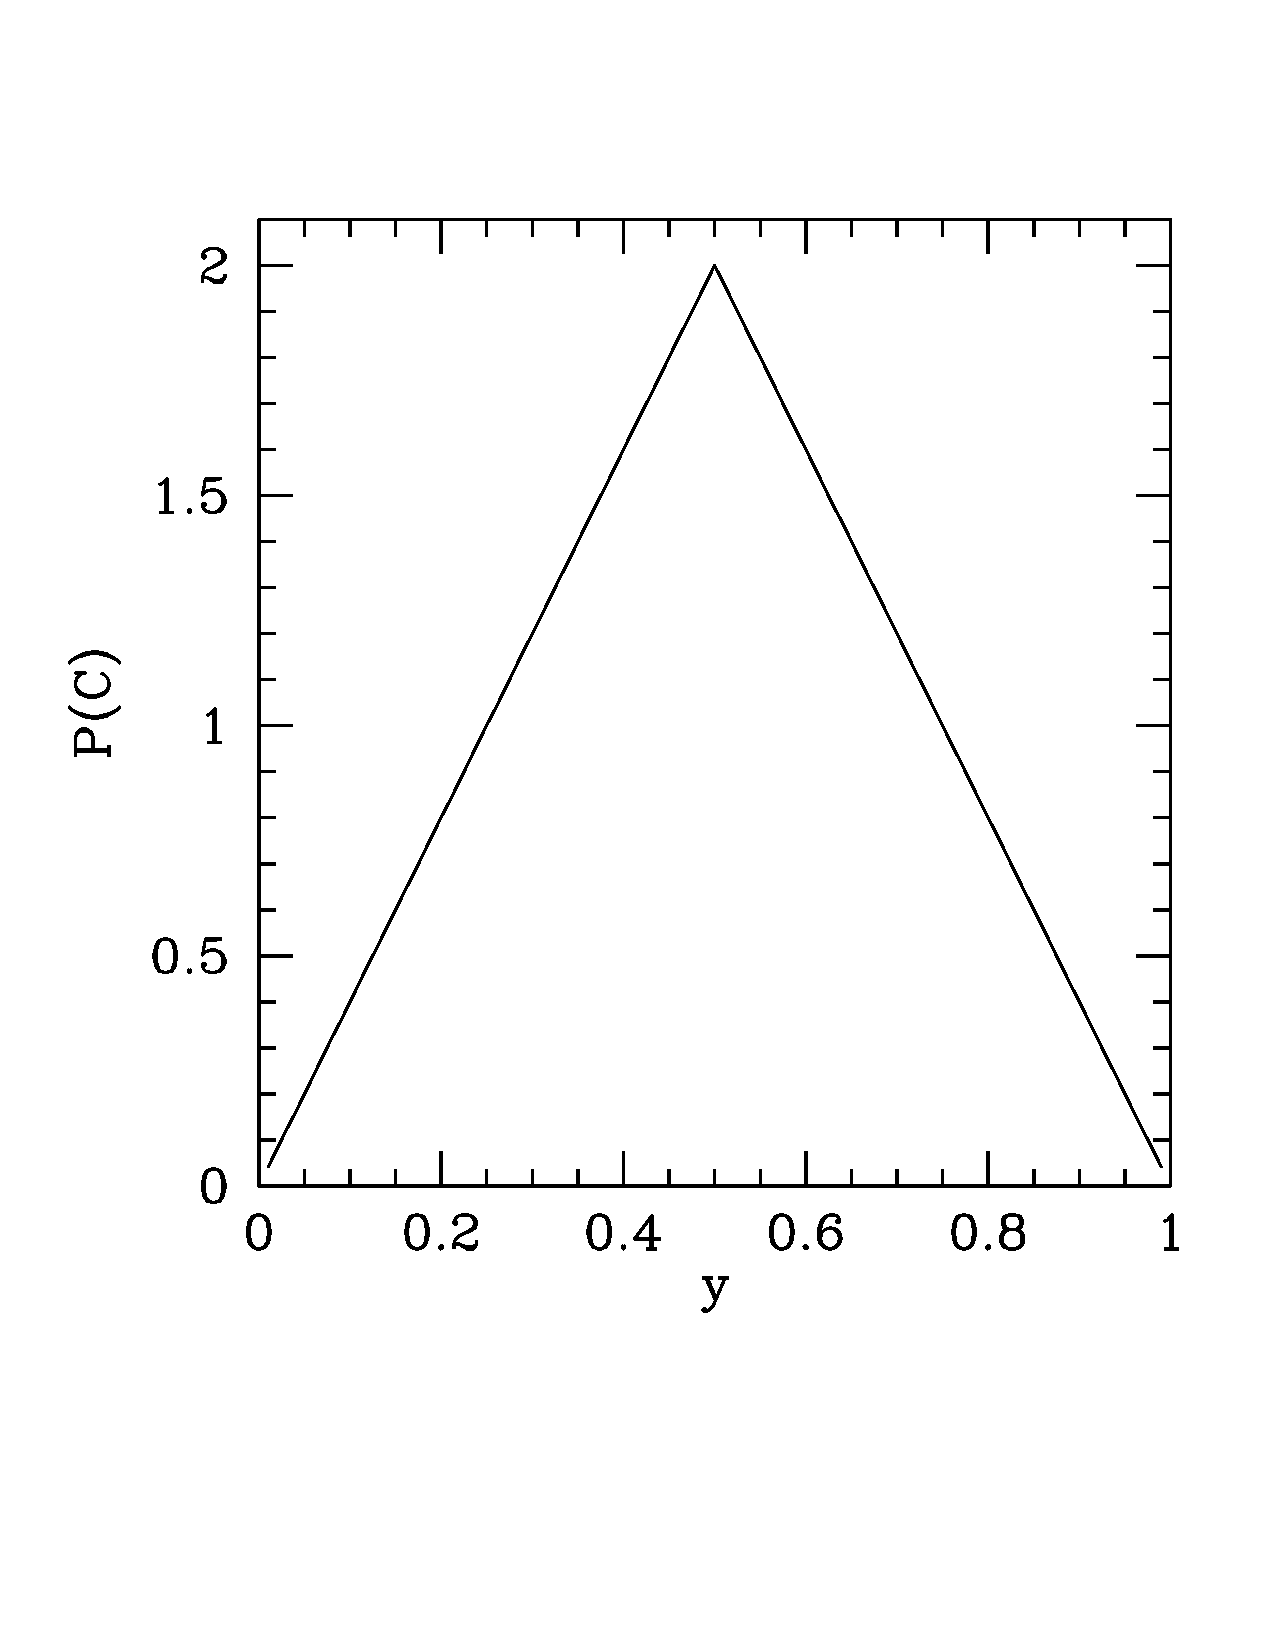
\includegraphics[width=0.45\textwidth]{fig_linear_prior_b}
  \end{center}
  \caption[Prior effect of a linear interpolation]{(a) Linear
  interpolation between two points $A, B$. $A, B$ are drawn from
  $[0,1]$ with uniform prior (b) The probability distribution of point
  $C$, located in the middle between $A$ and $B$.}
  \label{fig:linear_prior}
\end{figure*}
Using any expansion basis for interpolation, the prior distribution of
the spectral trajectories in between nodal points therefore is not
uniform either.

This effect can significantly alter the outcome of MCMC parameter
reconstruction runs as we will see below. Most prominently it can lead
to a spurious ``detection'' of tensors using the Chebyshev procedure
as all trajectory functions $\ptensor$ related to the
tensor scalar ratio $r$ are constrained to be positive.

Using B-splines as basis functions, we also find that the priors are
also heavily dependent on the order of the expansion and on the choice
of trajectory, i.e. whether we use $n_t$ or $\ptensor$ as
spectral trajectory. Figure~\ref{fig:prior_bspline} shows the prior
distribution of the tensor amplitude $\ptensor$ at
$k=0.002$Mpc$^{-1}$ for an $8$ parameter third order B-spline
expansion. It is immediately obvious that the apparent detection of
tensors (solid line) is solely caused by the prior (dashed line)
implied in this expansion.
\begin{figure*}
  (a)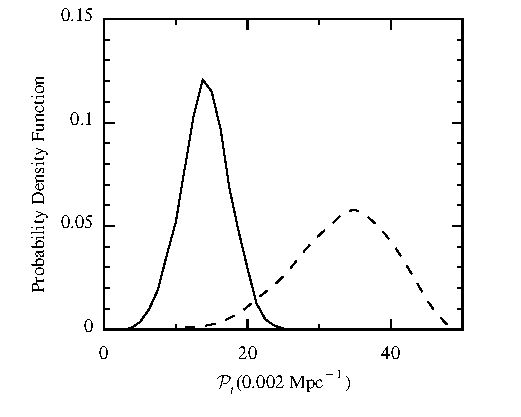
\includegraphics[width=0.45\textwidth]{prior_posterior_monopt}
  (b)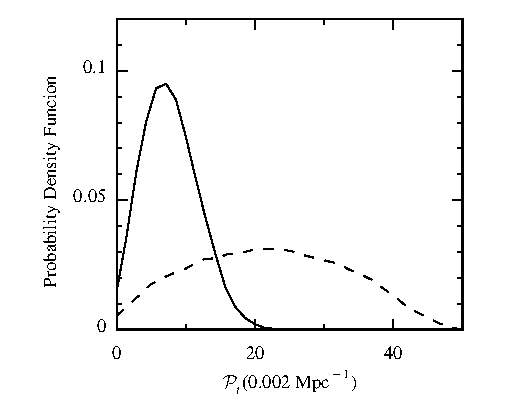
\includegraphics[width=0.45\textwidth]{prior_posterior_pt}
  \caption{Prior (dashed) and posterior (solid)
    distribution of the tensor power $\ptensor$ at
    $k=0.002$Mpc$^{-1}$ for an eight parameter B-spline expansion. The
    apparent detection of $r$ in the posterior is clearly an effect of
    the implicit prior. (a) monotonic $\ptensor$. (b)
    non-monotonic $\ptensor$.}
  \label{fig:prior_bspline}
\end{figure*}
Generating spectral trajectories $\ptensor$ without requiring
monotonicity, the prior shows a moderate favor for medium values,
caused by the interpolation effect mentioned above. The asymmetry
stems from the fact that the point $k=0.002$Mpc$^{-1}$ is not exactly
in the middle between two nodal points.

Enforcing monotonicity of $\ptensor$, the prior shows a strong
favor of large values (panel (a)). Two effects are responsible for
this: the interpolation effect as elaborated above, and the fact that
monotonicity makes the prior position dependent even at nodal points,
see Figure~\ref{fig:monotonicity}. If $\ptensor$ is monotonically
decreasing with $k$, the values at smaller $k$ must be larger on
average than the values at larger $k$. Going towards medium values of
$\ln k$, the distribution becomes uniform, and finally at large values
of $\ln k$, small values of $\ptensor$ are strongly favored.
\begin{figure}
  \begin{center}
    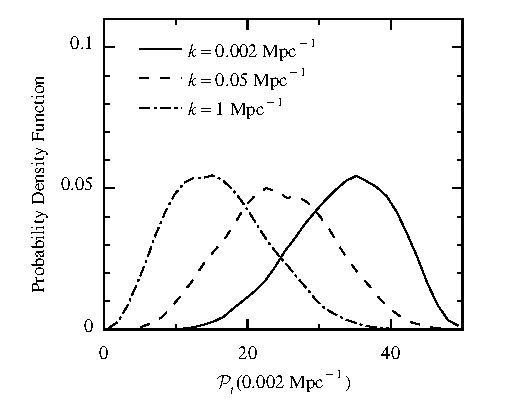
\includegraphics[width=0.45\textwidth]{prior_monopt}
  \end{center}
  \caption{Prior distribution of a monotonically decreasing trajectory
    $\ptensor$. Going from small values of $\ln k$ (solid) over
    intermediate (dashed) to large values of $\ln k$ (dashed-dotted),
    the distribution's shape changes significantly.}
  \label{fig:monotonicity}
\end{figure}
The point $k=0.002$Mpc$^{-1}$ lies in the left half of k-space,
therefore the prior favors larger values of the tensor amplitude.

The bottom line is that different parameterizations imply different
priors. When thinking about parameterizing the primordial spectra (or
any other quantity that is not well constrained by current
observational data), great care must be taken to accurately take into
account the effects of the priors.


\bibliographystyle{JHEP}  
\bibliography{scanning_bb}

\end{document}
